\documentclass[oneside]{book}
\usepackage[a4paper, total={6in, 8in}]{geometry}
\usepackage[english]{babel}
\usepackage[utf8]{inputenc}
\usepackage[T1]{fontenc}
\usepackage{cancel}
\usepackage{amsmath}
\usepackage{amsfonts}
\usepackage{dsfont}
\usepackage{listings}
\usepackage{hyperref}
\usepackage{siunitx}
\usepackage{fancyhdr}
\usepackage{textcomp}
\usepackage{makecell}
\usepackage[font=small,labelfont=bf]{caption}
\usepackage{pdfpages}
\usepackage{multicol}
\usepackage[ruled,vlined]{algorithm2e}
\usepackage{soul}
\usepackage{mhchem}
\usepackage[toc, page]{appendix}
\usepackage{float}
\usepackage{wrapfig}
\usepackage{braket}
\usepackage{xcolor}
\usepackage{mathtools}
\usepackage{physics}
\usepackage{multirow}
\usepackage{siunitx}
\pagestyle{fancy}
\fancyhf{}
\lhead{\rightmark}
\cfoot{\leftmark}
\rfoot{\thepage}
\usepackage[export]{adjustbox}
\usepackage{wrapfig}
\usepackage{float}

\setcounter{secnumdepth}{5}

\lstset{
    frame=tb, % draw a frame at the top and bottom of the code block
    tabsize=4, % tab space width
    showstringspaces=false, % don't mark spaces in strings
    numbers=none, % display line numbers on the left
    commentstyle=\color{green}, % comment color
    keywordstyle=\color{red}, % keyword color
    stringstyle=\color{blue}, % string color
    breaklines=true,
    postbreak=\mbox{\textcolor{green}{$\hookrightarrow$}\space}
}

\renewcommand{\lstlistingname}{}% Listing -> Algorithm
\renewcommand{\lstlistlistingname}{Algoritmi}% List of Listings -> List of Algorithms


\renewcommand*{\listalgorithmcfname}{}
\renewcommand*{\algorithmcfname}{}
\renewcommand*{\algorithmautorefname}{}
\renewcommand{\thealgocf}{}
\newcommand{\mathcolorbox}[2]{\colorbox{#1}{$\displaystyle #2$}}


\title{\Huge\textbf{{Computational biophysics}}}

\author{
  Giacomo Fantoni \\
  \small telegram: \href{https://t.me/GiacomoFantoni}{@GiacomoFantoni} \\[3pt]
  \small Github: \href{https://github.com/giacThePhantom/mathematical-modelling-in-biology}{https://github.com/giacThePhantom/mathematical-modelling-in-biology}\\
}


\begin{document}

  \maketitle
  \tableofcontents
  \chapter{Introduction and proteins}

  \graphicspath{{chapters/02/images/}}
\chapter{Proteins' geometry}

\section{Introduction}
The study of the geometry of proteins involve what can be learned from protein's coordinates.

\section{The peptide bond}
A protein is a collection of amino acids linked together by a peptide bond.
A carboxylic end and an amino end of two amino acid react together losing a water molecule and forming a peptide bond.
Beside the $\alpha$-carbon there is another one bonded to the oxygen in the carboxylic group and a nitrogen bond in the amino group.
The $\alpha$ carbon is linked to the nitrogen in the amino group of another amino acid.
The carbon and nitrogen display $sp2$ hybridization, the central atom and the $3$ that form a bond with it form a plane, so the peptide bond is planar.
A plane of the peptide bond is formed and rotation of the plane is allowed only around one axis.
\begin{figure}[H]
			\centering
			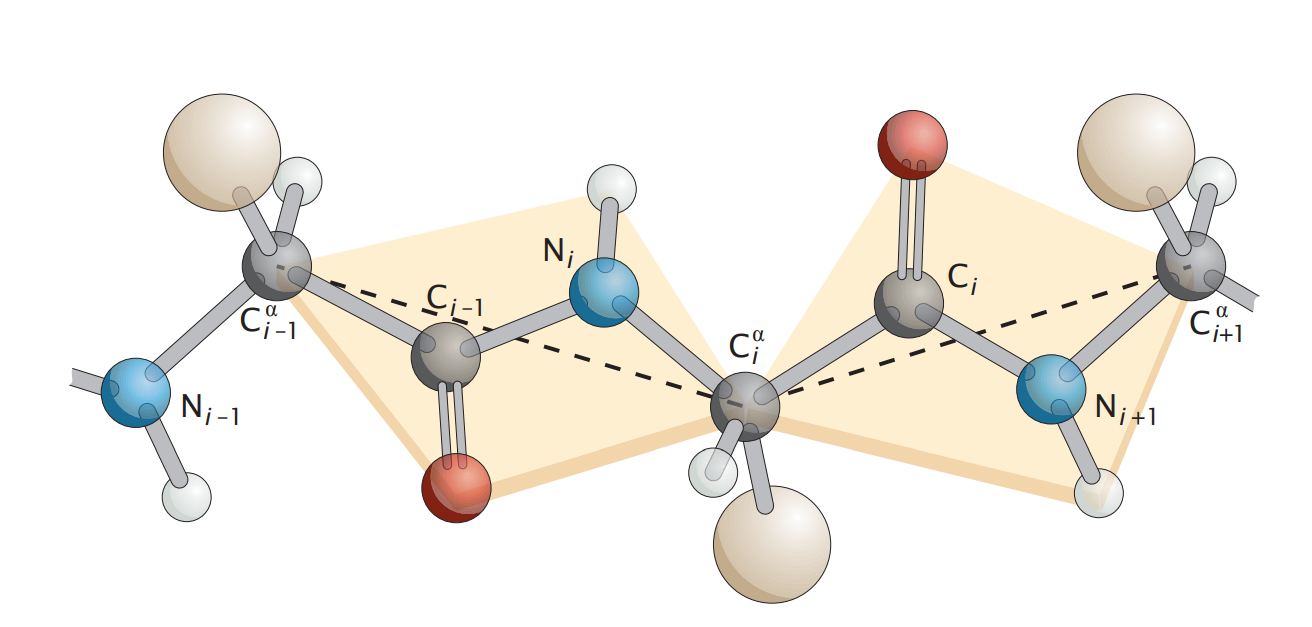
\includegraphics[width=\textwidth]{planar.png}
			\caption{sp2 hybridization of backbone C and N (not $C^{\alpha}$). This is an experimental finding which needs to be incorporated into the system: in this way (and by taking into consideration all the knowledge on proteins), the degree of freedom of the system can be reduced.}
			\label{fig:planar}
			\end{figure}

	\subsection{Trans and cis}
	Looking at the peptide bond the carbon atom of the carboxylic group $C'$ and the nitrogen $N$ are each bonded to a different $\alpha$-$C$ and a trans or cis conformation can happen.
	Trying to visualize the atoms that belong to the molecules these repel through the Van der Waals interactions, that can be computed through the Lennard-Jones potential (represented in figure \ref{fig:potential}):

	$$U_{Lj}(r) = E_0\biggl[\biggl(\frac{r_0}{r}\biggr)^{12}-2\biggl(\frac{r_0}{r}\biggr)^6\biggr]$$

	Where:

	\begin{multicols}{2}
		\begin{itemize}
			\item $r_0$ is the distance where the energy is minimum.
			\item $r$ is the distance between two atoms.
			\item $r_{min}$ is the distance at which the energy becomes high.
		\end{itemize}
	\end{multicols}

	\begin{figure}[H]
			\centering
			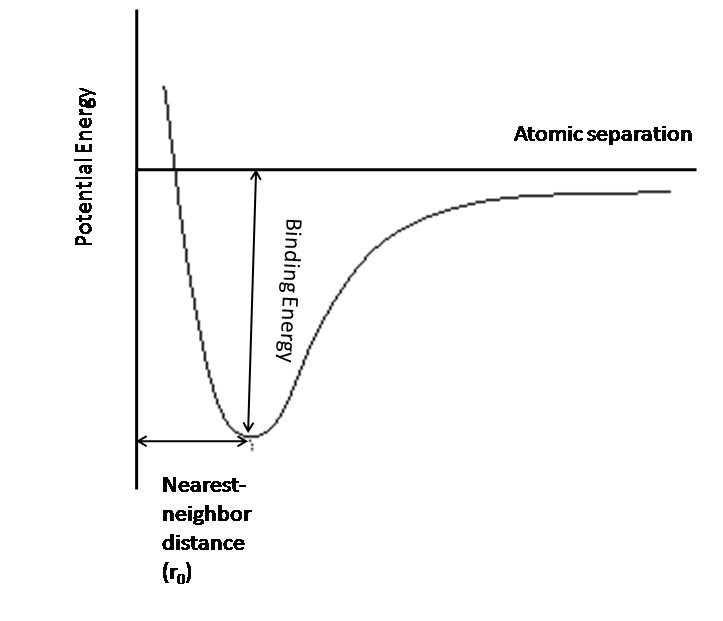
\includegraphics[width=\textwidth]{potential.png}
			\caption{Graphical representation of the energy plotted along the distance between atoms. $r_0$ is the equilibrium distance and it explains the reason why the trans configuration is preferred over the cis configuration}
			\label{fig:potential}
			\end{figure}

	With atoms most of the time the distance between them will be close to $r_0$.
	When decreasing the distance a lot of energy is needed and strain is introduced in the molecule.
	Plotting the values for the energy, $r_0$ and $r_{min}$ the expected distance for each couple of atoms can be seen.
	Focusing on the $C$-$C$ interaction:

	\begin{multicols}{2}
		\begin{itemize}
			\item $r_0 = 3.4\si{\angstrom}$.
			\item $r_{min} = 3.0\si{\angstrom}$.
		\end{itemize}
	\end{multicols}

	When two carbons atoms are below the minimum value the conformation is strained.
	Looking back at the conformation of the peptide bond it can be seen that the cis conformation creates a distance of $2.8\si{\angstrom}$ between the two $\alpha$-$C$, so it is not favourable.
	So the trans conformation is the least energy-hungry and the most present.

	Note that the Lennard-Jones potential is not the only one possible.
	Although it is preferred in most scenarios, other types of potential (e.g., buckingham potential or LJ with different powers) there exist.

\section{The Ramachandran angles}
The planes formed by the peptide bonds can rotate with respect to each other.
So the Ramachandran angles $\phi$ and $\psi$ can be defined between these planes.
For each $\alpha$-$C$:

\begin{multicols}{2}
	\begin{itemize}
		\item $\phi$ describes the rotation around its bond with the nitrogen.
		\item $\psi$ describes the rotation around its bond with the carboxylic group.
	\end{itemize}
\end{multicols}

These are the angles between the subsequent planes.
Some of the angles will require more energy.

	\subsection{Difficulty of rotation}
	It can be seen how a rotation of the $\phi$ angle could cause the two $C'$ to come at a distance of $2.9\si{\angstrom}$ (where $r_{min} = 3.0\si{\angstrom}$.
	On the other hand a rotation of the $\psi$ angle could cause the two $N$ to come at the same distance, but in this case $r_{min}(N-N) = 2.7\si{\angstrom}$.
	In the case of carbon atoms the distance is less than the minimum distance, while in the case of nitrogen it is greater than the minimum allowed value.
	Looking at this it can be seen how the $\psi$ rotation is easier.

	\subsection{Ramachandran plot}
	A Ramachandran plot is a map with the $\phi$ angle on the $x$ axis and the $\psi$ angle on the $y$ axis.
	Because a rotation along the $\phi$ angle is highly disfavoured the angle $0$ is strongly disfavoured and is represented like a black stripe (disallowed region).
	If the amino acids where composed only by carbon and nitrogen atom the Ramachandran map would be the one represented in figure \ref{fig:rama}, where it can be found:

	\begin{multicols}{2}
		\begin{itemize}
			\item A forbidden region in the middle.
			\item Some strained region like for $\psi=0$.
		\end{itemize}
	\end{multicols}

	\begin{figure}[H]
		\centering
		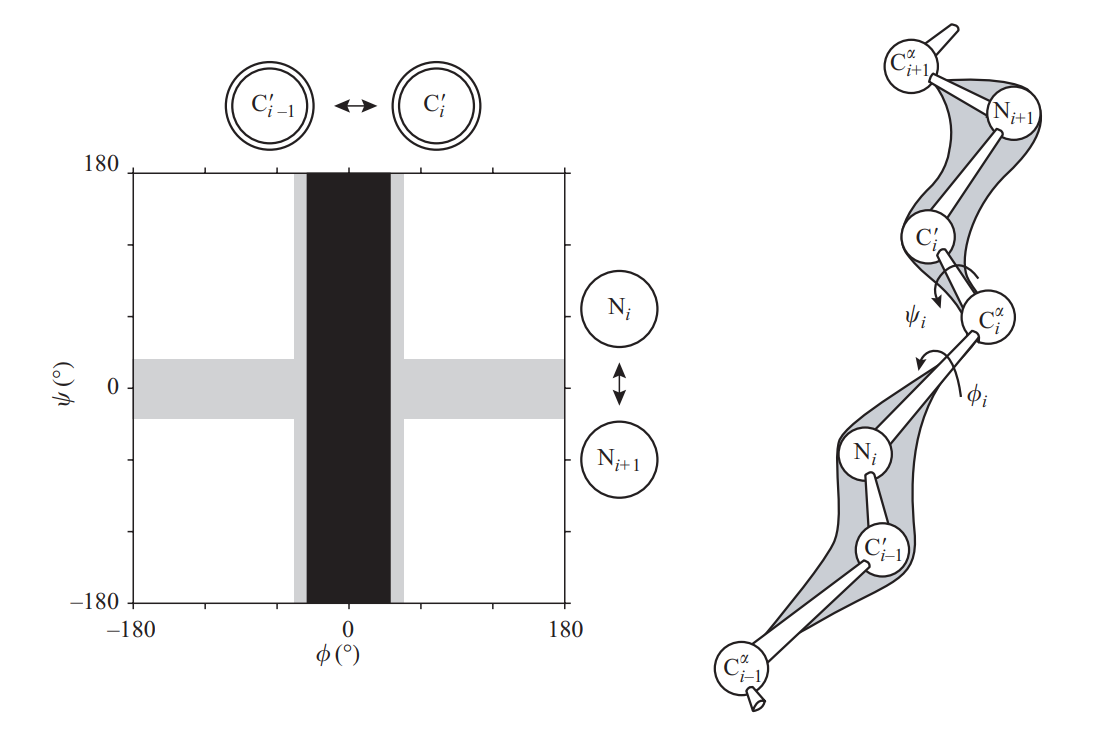
\includegraphics[width=\textwidth]{rama_map.png}
		\caption{This is how Ramachandran plots of the disallowed (black stripe), strained (grey stripe), and fully allowed (white regions) ($\phi$, $\psi$) conformations of the fragment $C^{\alpha}C'N$---$C^{\alpha}$---$C'N-C^{\alpha}$ would look, provided all these atoms had no other atoms attached (right) and atoms of residues $i-1$ and $i+1$ had no interactions.}
		\label{fig:rama}
	\end{figure}

	Looking at a real protein the complexity is increased and the other oxygen and nitrogen atoms are included \ref{fig:ramachandran-complex} and other regions become disallowed due to steady clashes.
	It can be seen how the regions are quite complex.

	\begin{figure}[H]
		\centering
		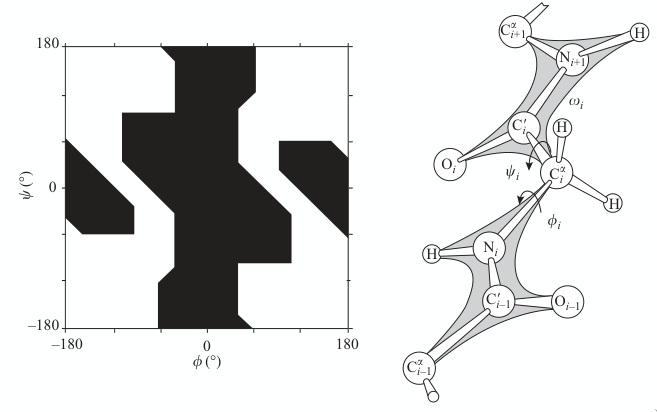
\includegraphics[width=\textwidth]{ramachandran-complex.png}
		\caption{Ramachandran plot of a peptide bond with other atoms.}
		\label{fig:ramachandran-complex}
	\end{figure}

		Looking at a glycine and alanine complex it can be seen in \ref{fig:ala_gly-theo} the space becomes even more complex.

	\begin{figure}[H]
		\centering
		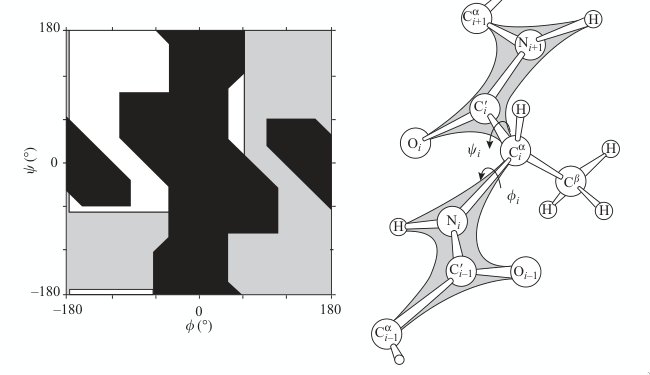
\includegraphics[width=\textwidth]{ala-gly-theo.png}
		\caption{Theoretical representation of a Ramachandran plot of a glycine-alanine complex.}
		\label{fig:ala_gly-theo}
	\end{figure}

	In this case the white regions is very small and a strained region can be seen and the black one.
	Including other residues the allowed region reduces \ref{fig:ramachandran-final}.
	This is due to the presence of larger residues.

	\begin{figure}[H]
		\centering
		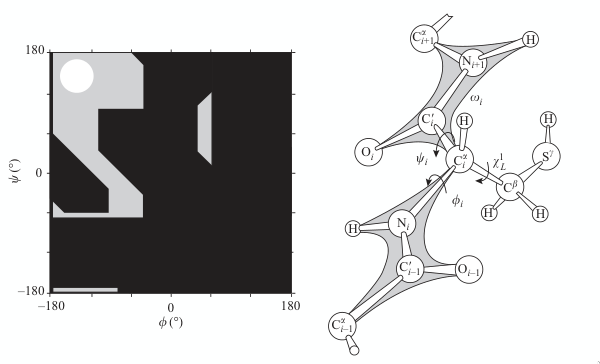
\includegraphics[width=\textwidth]{ramachandran-final.png}
		\caption{Ramachandran plot of a larger residue.}
		\label{fig:ramachandran-final}
	\end{figure}

		\subsubsection{Observed Ramachandran plot}
		Trying to plot for each amino acid its angles an amino acid is represented as a dot.
		Most of the points fall inside of the allowed regions but there are some outliers.
		In some conformation the protein forces the amino acid to assume strange conformations.
		This is done to check if the structure places the amino acids in a proper way.
		A typical observed Ramachandran plot looks like the one in \ref{fig:ala_gly}.

		\begin{figure}[H]
			\centering
			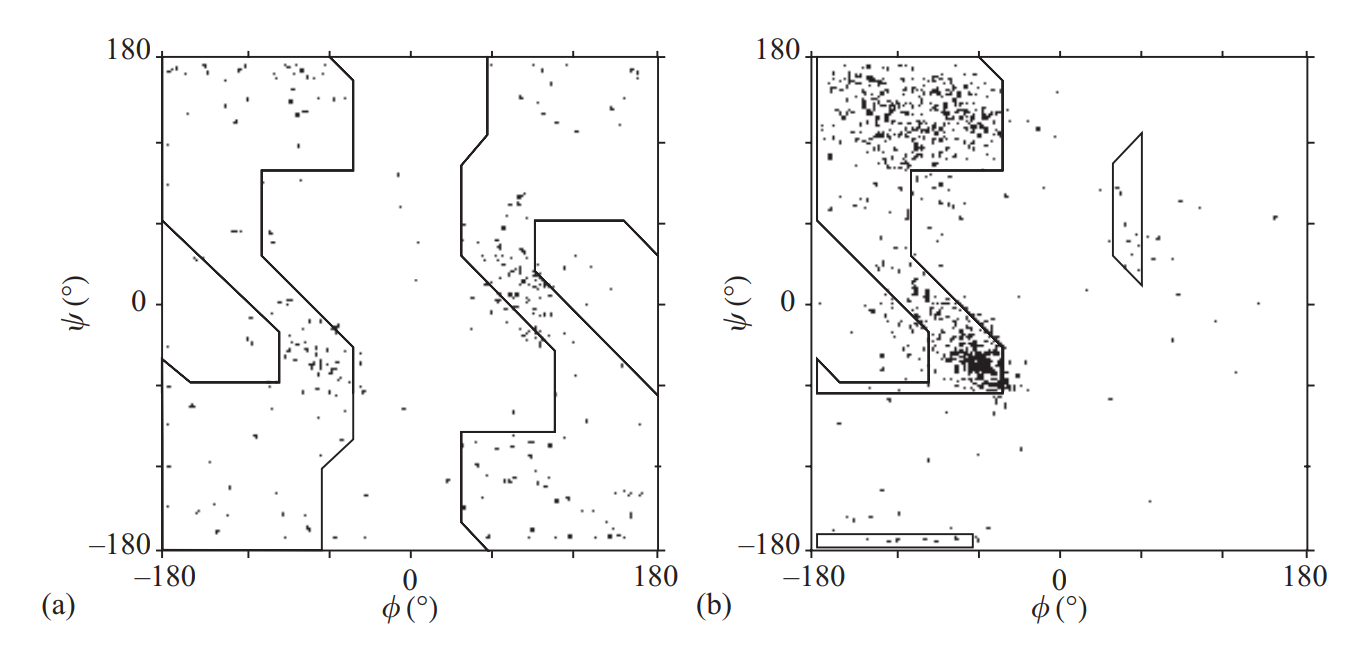
\includegraphics[width=\textwidth]{ala_gly.png}
			\caption{Observed conformations (dots) of glycine (a) and of other amino acid residues (b) in proteins. The sterically allowed regions are contoured.}
			\label{fig:ala_gly}
		\end{figure}


\section{Contact map of proteins}
Starting from the coordinates a contact map can be built.
It is a matrix that map all the contact between the amino acids.
A primary structure can be represented as a collection of beads which will be in contact in the 3D structure.
A square matrix can be built such that each entry in the matrix will determine whether there is a contact or not.
This matrix will be symmetric with diagonal elements with value $1$ and two parallel diagonals for the neighbouring amino acids (figure \ref{fig:contact}).
Secondary structures will have specific signatures:

\begin{multicols}{2}
	\begin{itemize}
		\item $\alpha$-helices: is usually represented by a line parallel to the diagonal.
			This is because the amino acids $i$ is interacting with $i+4$.
		\item $\beta$-strands: the situation is complicated.
			For parallel $\beta$ sheets can be parallel to the diagonal.
			For anti-parallel it can be anti-parallel to the diagonal.
	\end{itemize}
\end{multicols}


\begin{figure}[H]
			\centering
			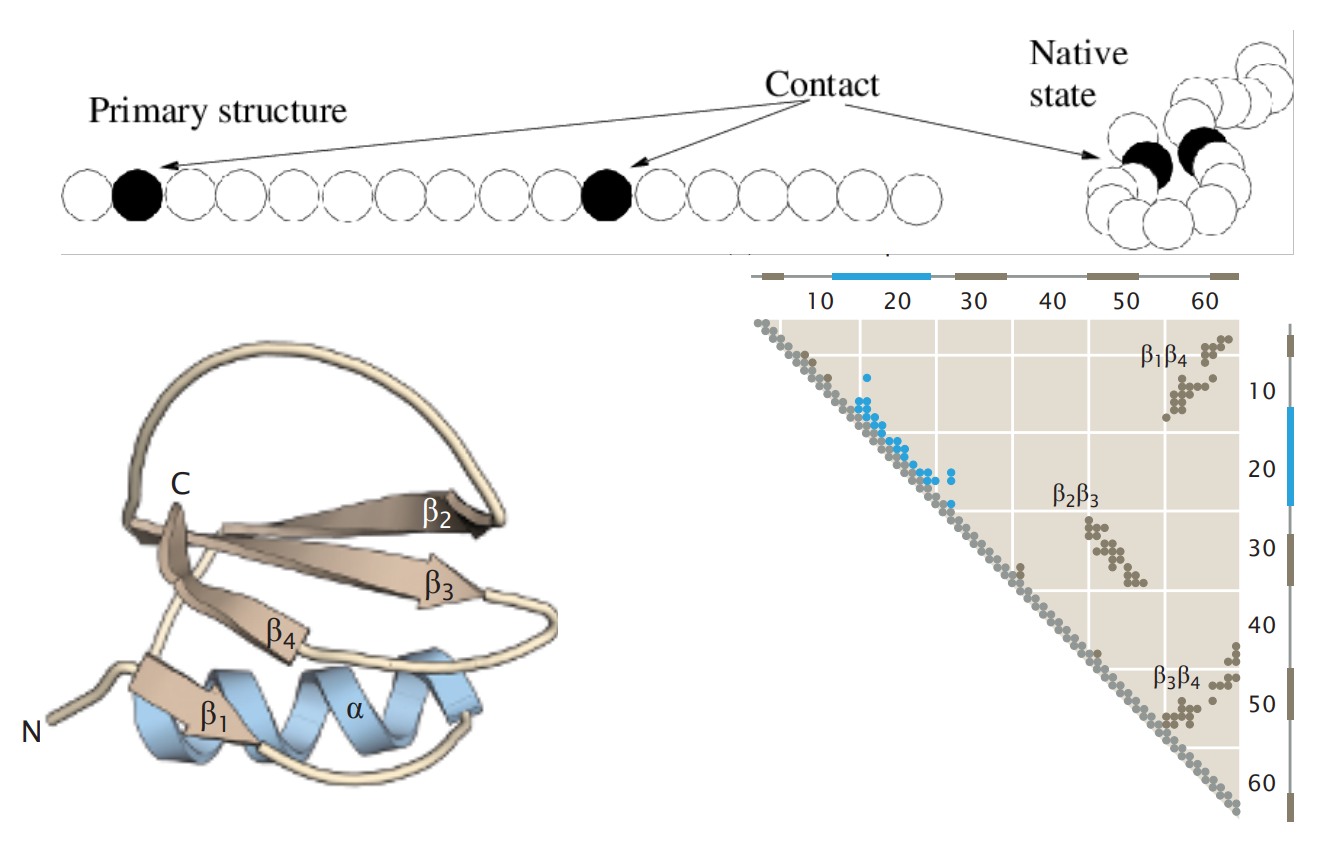
\includegraphics[width=\textwidth]{contact.png}
			\caption{Example of a contact map for a protein.}
			\label{fig:contact}
			\end{figure}


	\subsection{Defining a contact}
	The contact between two amino acids needs to be defined.
	To do so the distance between $\alpha$-$C$ or the distance between the tail of the residue and an $\alpha$-$C$.
	There is also the need to make a trade-off between computational speed and cost.
	Also the dimension of the protein need to be considered when choosing the distance.

\section{Topology diagram}
Having found the secondary structures with a contact map a topology diagram help to understand how those interact with each other (figure \ref{fig:topology}).
In a topology diagram the start is the $N$ terminus and the end the $C$ terminus.
$\beta$-strands are represented as arrows.
If the strands always change direction they will form an anti-parallel $\beta$-sheet.
$\alpha$-helices are represented as small cylinder.
Usually color codes represent the nature of the structure.
This helps with numbering of the secondary structures.

\begin{figure}[H]
			\centering
			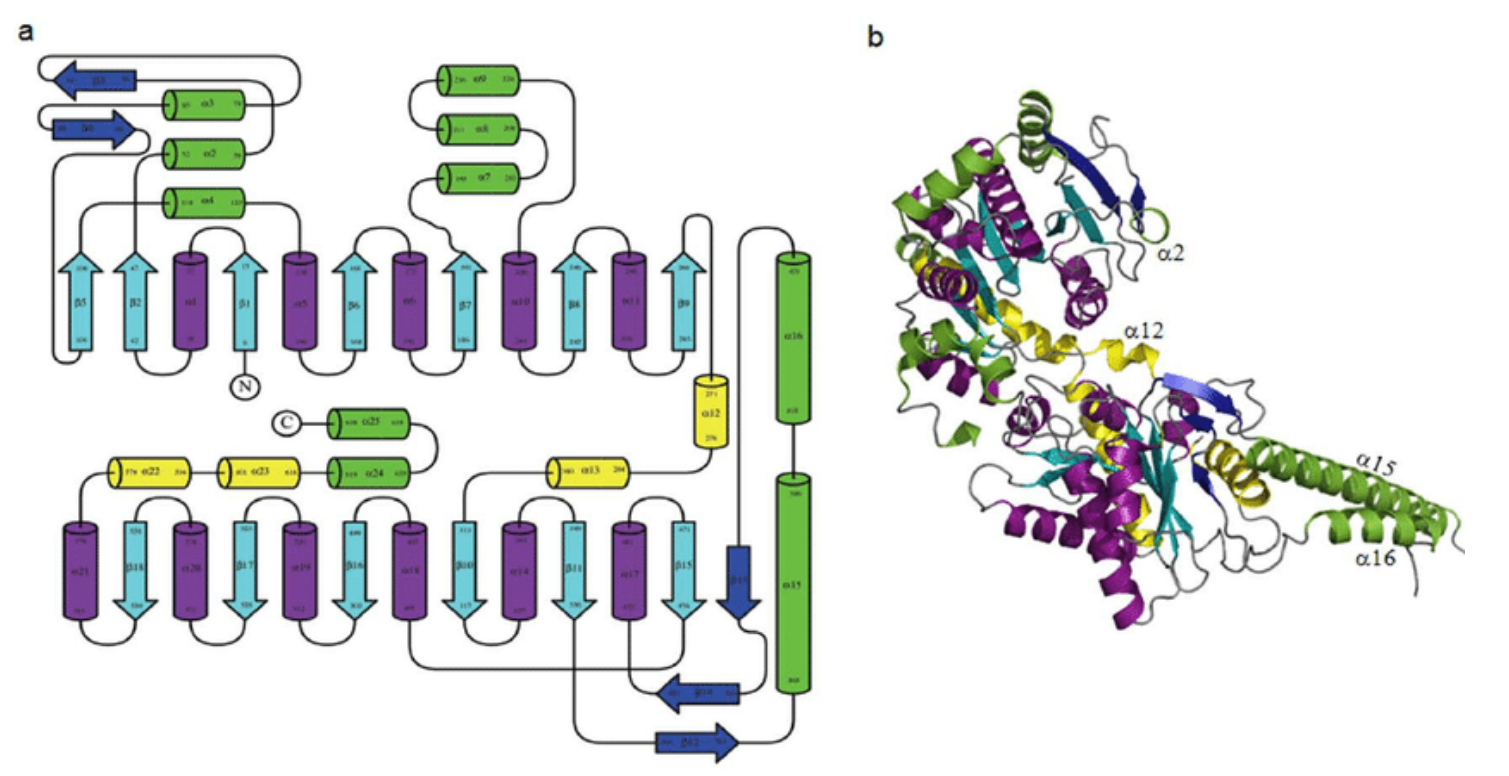
\includegraphics[width=\textwidth]{topology.png}
			\caption{The topology of a protein structure is a highly simplified description of its fold including only the sequence of secondary structure elements, and their relative spatial positions and approximate orientations. This information can be embodied in a two-dimensional diagram of protein topology, called a TOPS cartoon. (from pubmed)}
			\label{fig:topology}
			\end{figure}


\section{Coordinates}
The coordinates of all atoms in a protein are described in a PDB file.
This is a tabulated file containing different columns:

\begin{multicols}{2}
	\begin{itemize}
		\item Atom record: ATOM.
		\item Atom number: a unique identifier for the atom.
		\item Atom identifier: an identifier for the type of atom.
		\item Amino type: the amino acid from which the atom is from.
		\item Chain identifier: identifier for the chain.
		\item Residue sequence number: the number of the residue in the chain.
		\item $x$, $y$, $z$: the coordinates in angstrom.
		\item Occupancy: the probability of an atom to be in that space (confidence space).
		\item B-factor: how mobile that atom is in the crystal, it represent the noise in the x-ray diffraction map (it represents the fluctuations for the coordinate of the atoms. For example, loops in trans-membrane proteins are very mobile and a high B-factor is to be expected).
		\item Element symbol: the symbol of the element of the atom.
	\end{itemize}
\end{multicols}

Once the coordinates of a protein is obtained, some geometrical properties can be directly computed.

	\subsection{Protein center of mass}
	The protein center of mass is the average position for the protein center.
	It is an average weighted by the mass of the atom.

	$$\vec{R}_{cm} = \frac{\sum\limits_{i=1}^Nm_i\vec{r}_i}{\sum\limits_{i=1}^Nm_i}$$

	\subsection{Radius of gyration}
	Once the center of mass is known the radius of gyration can be computed.
	This measures the size of the protein as if it was a sphere.
	It is a good indication of the globular size of a protein.
	It also indicates an elongating/shrinking behavior, and useful to check whether a protein is going toward equilibrium in the simulation.
	The distance of each atom and the center of mass is computed and the square is taken, weighted with the mass of the atom.

	$$R_g = \sqrt{\frac{\sum\limits_{i=1}^Nm_i(\vec{r}_i-\vec{R}_{cm})^2}{\sum\limits_{i=1}^Nm_i}}$$

	\subsection{Comparing protein structures}
	Proteins have structures that loop in a similar way, with similar regions within each other.
	To quantify the similarity between the protein structure a procedure needs to be followed:

		\begin{itemize}
			\item Select common regions: a $1$-$1$ correspondence between amino acid need to be found: the parts present only in one protein are not considered.
				A correspondence is built between the common regions on the single amino-acids.
				These can be different, usually the coordinates are confronted between the $\alpha$-$C$ atom and the residue is not considered.
				One of the things that can be done is to look at the secondary structures and add loops only when they look similar.
			\item Align the two structures: compute the centre of mass of the two proteins and translate the proteins so the centre of masses coincide.
			\item Finding the optimal rotation: the principal axes are computed and the proteins are rotated so that they superimpose.
				Once the optimal rotation is obtained the difference can be quantified.
			\item Compute RMSD (root mean square deviation): take the coordinates of the amino-acid $i$ in protein $A$ and $B$, their squared difference is computed and an average over all amino acid is computed and squared:

				$$RMSD = \sqrt{\frac{1}{N}\sum\limits_{i=1}^N(\vec{r}_{Ai}-\vec{r}_{Bi})^2}$$
				the RMSD is a length, usually in angstrom scale.
				This can be done for two proteins or for the protein taken at two different time step in a molecular dynamics simulation:

				$$RMSD(t) = \sqrt{\frac{1}{N}\sum\limits_{i=1}^N(\vec{r}_{i}(t)-\vec{r}_{i}(0))^2}$$

				Now the $RMSD$ can be plotted with respect to time.
				It can be seen how at $t=0$ $RMSD=0$ and after the value will increase.
				When the number reaches a plateau the protein should be in equilibrium.
				The plateau can jump to another value, meaning that the state is a meta-stable state of the protein, or the protein has more stable states or a loop is making something.
				This value is assigned to very complicated structures and different structures can have the same $RMSD$.
				Clearly, a reference structure needs to be picked.
				In MD of a protein evolving in time, the reference structure is the initial configuration of the protein.
				One can also decide to focus on a specific region.
				The $RMSD$ is an indicator of equilibrium: it is a necessary but not sufficient condition.
		\end{itemize}

		\begin{figure}[H]
			\centering
			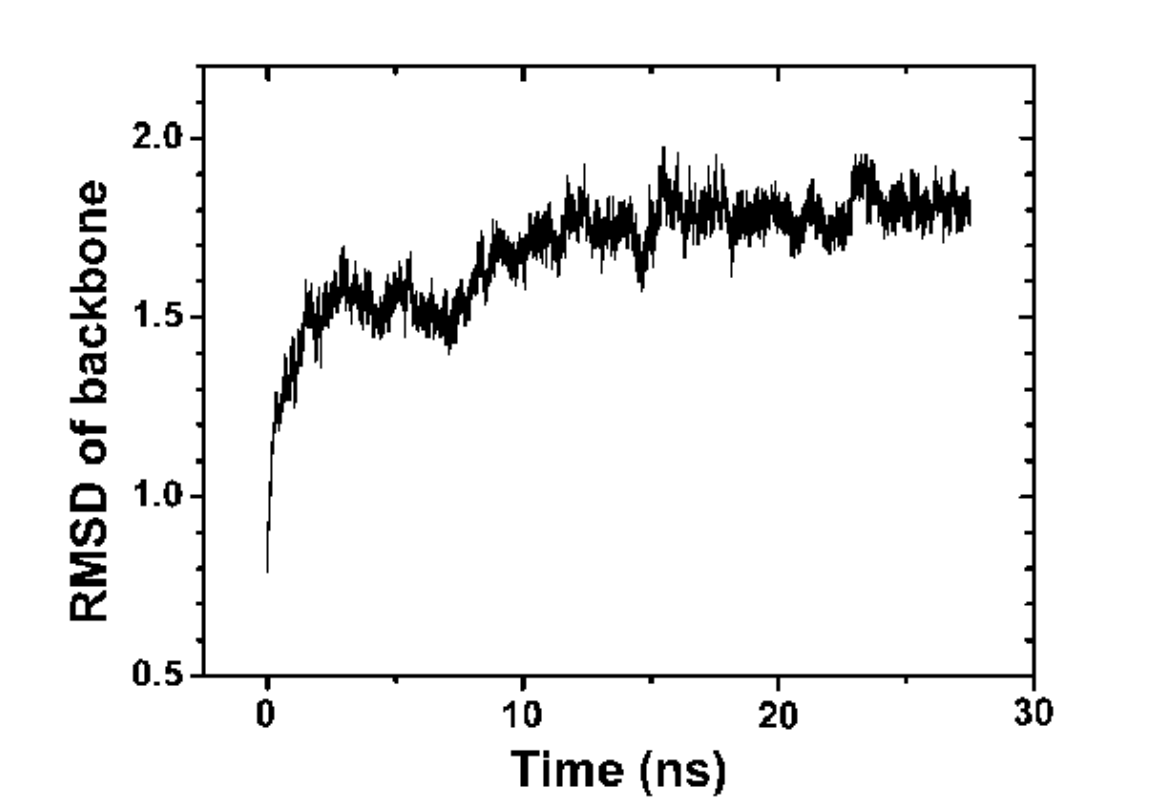
\includegraphics[width=\textwidth]{rmsd.png}
			\caption{RMSD of the backbone ($C^{\alpha}$, $N$, ...). We can see the typical steep jump a fluctuations towards the end of the plot. However, this is not enough to state that the protein reached equilibrium.}
			\label{fig:rmsd}
			\end{figure}


	\subsection{Native state}
	The native state is the functional state of a protein.
	It is not the state found for a crystallized protein, but only closely related to it, it is rather an ensemble in space and time of structures.
	This is due to proximity effect and the fact that the protein is not a static system.
	Proteins are extremely flexible and are moving a lot because the temperature corresponds to a constant movement of water molecule around causes movement in the protein.
	The native state is an ensemble of closely related states, all compatible with the conditions of the situation studied.
	Proteins need to be studied in the isothermal-isobaric ensemble.
	All the calculation need to be done at constant temperature and pressure.
	The native state is so a collection of functional state.

	In the case of the unfolded state the possibilities are too many to sample all of them.

	\subsection{RMSF}
	The flexibility of each amino acid can be computed.
	With flexibility is intended the movement of amino acid with respect to one another.
	In the $\alpha$-helix, for example, less fluctuation is expected, while in loops more fluctuation is expected.
	This quantity is computed in the root mean squared fluctuation, which will be computed for each amino acid in the protein.
	With $f$ referring to the frame, let:

	\begin{itemize}
		\item $\langle \vec{r}_i\rangle = \frac{1}{M}\sum\limits_{f=1}^M\vec{r}_{i,f}$, the average position of atom $i$.
		\item $\Delta\vec{r}_{i,f} = \vec{r}_{i,f}-\langle\vec{r}_i\rangle$, the displacement of each atom in each frame with respect to its average.
		\item $\langle \Delta\vec{r}_o^w\rangle = \frac{1}{M}\sum\limits_{f=1}^M(\vec{r}_{i,f}-\langle\vec{r}_i\rangle)^2$, the average squared distance over the frames.
	\end{itemize}

	So, the root mean squared fluctuation is:

	$$RMSF_i = \sqrt{\langle\Delta\vec{r}_i\rangle^2}$$

	Plotting the $RMSF$ with respect to residue number and the more mobile residue can be identified.
	This can be mapped onto the sequence so loops, helices and strands can be recognized.
	Usually the fluctuating part correspond to loops.
	The terminus have the highest $RMSF$.

		\subsubsection{B-factors}
		$RMSF$ can be translated into B-factors.
		They are the Debye-Waller factors and are a scaled version of the $RMSF$ squared.
		So the result of a simulation can be compared with the B-factor and a strong correspondence can be seen.
		The differences are due to the fact that the crystal is a different environment with respect to the normal one and packing effect can happen (some regions of the protein can interact with the image of the protein in the crystal).

		$$B_i = \frac{8\pi^2}{3}\langle\Delta\vec{r}_i^2\rangle = \frac{8\pi^2}{3}RMSF^2_i$$

  \chapter{Force fields}

  \chapter{Classical mechanics}

\section{Newton's laws}

$$m_i\frac{d^2 \vec{r}_i}{dt^2} = m_i\ddot{\vec{r}}_i = \vec{F}_i$$

Then the forces:

$$\vec{F}_i(\vec{r}_1, \dots, \vec{r}_N, \dot{\vec{r}}_i) = \sum\limits_{j\neq i}\vec{f}_{ij}(\vec{r}_i-\vec{r}_j)+\vec{f}^{(ext)}(\vec{r}_i, \dot{\vec{r}}_i)$$

Now considering the energy already described:

\begin{multicols}{2}
	\begin{itemize}
		\item Bond stretching: $U = \frac{k_l}{2}(l-l^0)^2$.
		\item Bond bending: $U = \frac{k_\theta}{2}(\theta-\theta^0)^2$.
		\item Bond torsion: $U = k_\phi[1+\cos(n\phi-\phi^0)]$.
		\item Van der Waals interactions: $U = \biggl[\frac{a_{ij}}{r_{ij}^{12}}-\frac{b_{ij}}{r_{ij}^6}\biggr]$.
		\item Electrostatic interactions: $U = \frac{332q_iq_j}{\epsilon r_{ij}}$.
	\end{itemize}
\end{multicols}

	\subsection{Phase space}
	Consider the particle momenta:

	$$\vec{p}_i = m_i\vec{v}_i = m_i\dot{\vec{r}}_i$$

	And Newton's laws:

	$$\vec{F}_i = m_i\ddot{\vec{r}}_i = \dot{\vec{p}}_i$$

	Then the full dynamics of a system is specified by $6N$ functions, where $N$ is the numbers of the body in the system:

	$$\{\vec{r}_1(t), \dots, \vec{r}_N(t), \vec{p}_1(t), \dots, \vec{p}_N(t)\}$$

	And the microscopic state at time $t$ is specified by $6N$ numbers, the phase space vector:

	$$\vec{x} + \{\vec{r}_1, \dots, \vec{r}_N, \vec{p}_1, \dots, \vec{p}_N\}$$

	And the trajectory:

	$$\vec{x}_t = \{\vec{r}_1(t), \dots, \vec{r}_N(t), \vec{p}_1(t), \dots, \vec{p}_N(t)\}$$

	\subsection{One particle in one dimension}

		\subsubsection{Free particle}

		\subsubsection{Harmonic oscillator}
		On the harmonic oscillator:

		$$m\ddot{x} = -kx$$

		And

		$$\omega = \sqrt{\frac{k}{m}}$$

		Then for an elliptic trajectory with radiuses: $(2mC)^{frac{1}{2}}$ and $(2\frac{C}{m}\omega^2)^{\frac{1}{2}}$, thn the trajectory is:
		$$x(t) = x(0)\cos\omega t+ \frac{p(0)}{m\omega}\sin\omega t$$

		And:

		$$\frac{p^2(t)}{2m} +\frac{1}{2}m\omega^2x^2(t) = C$$

		\subsubsection{Hill potential}

\section{Lagrangian formulation}

Consider the conservative forces:

$$\vec{F}_i(\vec{r}_1, \dots, \vec{r}_N) = -\nabla_i U(\vec{r}_1, \dots, r_N)$$

And the work for the conservative forces:

$$W_{AB} = \int_A^B\vec{F}_id\vec{l} = U_A-U_B = -\Delta U_{AB}$$

And on closed pathways:

$$\oint\vec{F}_id\vec{l} = 0$$

The kinetic energy:

$$K(\dot{\vec{r}}_1, \dots, \dot{\vec{r}}_N) = \frac{1}{2}\sum\limits_im_i\dot{\vec{r}}_i^2$$

And the Lagrangian:

$$\mathcal{L}(\vec{r}_1, \dots, \vec{r}_N, \dot{\vec{r}}_1, \dots, \dot{\vec{r}}_N) = K(\dot{\vec{r}}_1, \dots, \dot{\vec{r}}_N)- U(\vec{r}_1, \dots, \vec{r}_N)$$

	\subsection{Euler-Lagrange equations}

	$$\frac{d}{dt}\biggl(\frac{\partial\mathcal{L}}{\partial \dot{\vec{r}}_i}\biggr)-\frac{\partial\mathcal{L}}{\partial r_i} = 0$$

	Now:

	$$\mathcal{L} = \frac{1}{2}\sum\limits_i m_i\dot{\vec{r}}_i^2 - U(\vec{r}_1, \dots, \vec{r}_N)$$

	And:

	$$\frac{\partial\mathcal{L}}{\partial\dot{\vec{r}}_i} = m_i\dot{\vec{r}}_i$$

	$$\frac{\partial\mathcal{L}}{\partial\vec{r}_i} = -\frac{\partial U}{\partial\vec{r}_i}$$

	So that:

	$$m_i\ddot{\vec{r}}_i +\frac{\partial U}{\partial\vec{r}_i} = 0\rightarrow m_i\ddot{\vec{r}}_i = \vec{F}_i$$

		\subsubsection{Harmonic oscillator}
		Considering for example the harmonic oscillator the Lagrangian will be:

		$$\mathcal{L}(x, \dot{x}) = \frac{1}{2}m\dot{x}^2-\frac{1}{2}kx^2$$

		And:

		$$\frac{d}{dt}(m\dot{x}) + kx = 0\Rightarrow m\ddot{x} - kx$$

	\subsection{Conservation of energy}
	Let the equation of the energy:

	$$E = \frac{1}{@}\sum\limits_{i}m_i\dot{\vec{r}}_i^2 + U(\vec{r}_i, \dots, \vec{r}_N)$$

	Then:

	\begin{align*}
		\frac{dE}{dt}&= \sum\limits_im_i\dot{\vec{r}}_i\ddot{\vec{r}}_i + \sum\limits_i\frac{\partial U}{\partial \vec{r}_i}\dot{\vec{r}}_i=\\
								 &=\sum\limits_i\dot{\vec{r}}_i\biggl[m_i\ddot{\vec{r}}_i+\frac{\partial U}{\partial\vec{r}_i}\biggr] = \\
								 &=\sum\limits_i\dot{\vec{r}}_i[m_i\ddot{vec{r}}_i-\vec{F}_i] = 0
	\end{align*}

	\subsection{Generalized coordinates}
	Let the generalized coordinates:

	\begin{align*}
			q_\alpha &= f_\alpha(\vec{r_1}, \dots, \vec{r}_N)\qquad \alpha &= 1, \dots, 3N\\
			\vec{r}_i &=\vec{g}_i(q_1, d\dots, q_{3N}) i &=1, \dots, N
	\end{align*}

	Then:

	$$\dot{\vec{r}}_i = \sum\limits_{\alpha=1}^{3N}\frac{\partial \vec{r}_i}{\partial q_\alpha}\dot{q}_\alpha$$

	And let:

	$$\tilde{K}(q, \dot{q}) = \frac{1}{2}\sum\limits_{\alpha=1}^{3N}\sum\limits{\beta=1}^{3N}\biggl[\sum\limits_{i=1}^Nm_i\frac{\partial\vec{r}_i}{\partial q_\alpha}\frac{\partial\vec{r}_i}{\partial q_\beta}\biggr]\dot{q}_\alpha\dot{q}_\beta$$

	And introducing the mteric mass tensor $G_{\alpha\beta} = \biggl[\sum\limits_{i=1}^Nm_i\frac{\partial\vec{r}_i}{\partial q_\alpha}\frac{\partial\vec{r}_i}{\partial q_\beta}\biggr]$:

	$$\tilde{K}(q, \dot{q}) = \frac{1}{2}\sum\limits_{\alpha=1}^{3N}\sum\limits{\beta=1}^{3N}G_{\alpha\beta}\dot{q}_\alpha\dot{q}_\beta$$

	Then the Lagrangian in generalized coordinates becomes:

	$$\mathcal{L}(q, \dot{q}) =\frac{1}{2}\sum\limits_{\alpha=1}^{3N}\sum\limits{\beta=1}^{3N}G_{\alpha\beta}\dot{q}_\alpha\dot{q}_\beta - U(q_1, \dots, q_{3N})$$

	And the Euler-Lagrange equations:

	$$\frac{d}{dt}\biggl(\frac{\partial\mathcal{L}}{\partial\dot{q}_\alpha}\biggr) -\frac{\partial\mathcal{L}}{\partial q_\alpha} = 0$$

	\subsection{Legendre transforms}
	The aim of a Legendre transform is to express the function $f(x)$ in terms of its first derivative $s$:

	$$s = f'(x) \equiv g(x)$$

	Then:

	$$f(x_0) = f'(x_0)x_o + b(x_0)$$

	And:

	$$f(x) = f'(x)x+b(x)$$

	But:

	$$f'(x) = g(x) = s \Rightarrow x = g^{-1}(s)$$

	Hence $b(x)$ contains the same information as $f(x)$, however:

	$$b(g^{-1}(s)) = f(g^{-1}(s))-sg^{-1}(s) \equiv\tilde{f}(s)$$

	The Legendre transom is then:

	$$\tilde{f}(s) = f(x(s))-sx(s)$$

		\subsubsection{Legendre transform for multiple variables}
		Considering $n$ variables:

		$$s_1 = \frac{\partial f}{\partial x_1} = g_1(x_1, \dots, x_n), \dots, s_n = \frac{\partial f}{\partial x_n} = g_1(x_1, \dots, x_n)$$

		So the Legendre transform:

		$$\tilde{f}(s_1, \dots, s_n) = f(x_1(s_1, \dots, s_n), \dots, x_n(s_1, \dots, s_n))-\sum\limits_i s_ix_i(s_1, \dots, s_n)$$

		This holds for a subset of variables.

\section{Hamiltonian formulation}
Consider:

$$\vec{p}_i\equiv\frac{\partial\mathcal{L}}{\partial\dot{\vec{r}}_i} = \frac{\partial}{\partial\dot{\vec{r}}_i}\biggl[\frac{1}{2}\sum\limits_{j=1}^Nm_j\dot{\vec{r}}_j^2 - U(\vec{r}_1, \dots, \vec{r}_N)\biggr] = m_i\dot{\vec{r}}_i$$

Considering the Legendre transform of the Lagrangian:

\begin{align*}
	\tilde{\mathcal{L}}(\vec{r}_1, \dots, \vec{r}_N, \vec{p}_1, \dots, \vec{p}_N) &= \mathcal{L}(\vec{r}_1, \dots, \vec{r}_N, \dot{\vec{r}}_1(\vec{p}_1), \dots, \dot{\vec{r}}_N(\vec{p}_N))-\sum\limits_{i}\vec{p}_i\dot{\vec{r}}_i(\vec{p}_i) = \\
																																								&=\frac{1}{2}\sum\limits_{i=1}^Nm_i\biggl(\frac{\vec{p}_i}{m_i}\biggr)^2-U(\vec{r}_1, \dots, \vec{r}_N)-\sum\limits_{i=1}^N\vec{p}_i\frac{\vec{p}_i}{m_i} = \\
																																								&=-\sum\limits_{i=1}^N\frac{\vec{p}_i^2}{2m_i} - U(\vec{r}_1, \dots, \vec{r}_N)
\end{align*}

Now let:

$$\mathcal{H}(\vec{r}_1, \dots, \vec{r}_N, \vec{p}_1, \dots, \vec{p}_N) = -\tilde{\mathcal{L}}(\vec{r}_1, \dots, \vec{r}_N, \vec{p}_1, \dots, \vec{p}_N)$$

So that:

$$\mathcal{H}(\vec{r}_1, \dots, \vec{r}_N, \vec{p}_1, \dots, \vec{p}_N) = \sum\limits_i\vec{p}_i\dot{\vec{r}}_i(\vec{p}_i) - \mathcal{L}(\vec{r}_1, \dots, \vec{r}_N, \dot{\vec{r}}(\vec{p}_1), \dots, \dot{\vec{r}}_N(\vec{p}_N))$$

And:

$$\mathcal{H}(\vec{r}_1, \dots, \vec{r}_N, \vec{p}_1, \dots, \vec{p}_N) = \sum\limits_{i=1}^N\frac{\vec{p}_i^2}{2m_i} + U(\vec{r}_1, \dots, \vec{r}_N)$$

	\subsection{Generalized coordinates}
	Consider the generalized coordinates:

	$$p_\alpha = \frac{\partial\mathcal{L}}{\partial\dot{q}_\alpha} = \sum\limits_\beta G_{\alpha\beta}\dot{q}_\beta\Rightarrow \dot{q}_\alpha = \sum\limits_\beta G^{-1}_{\alpha\beta}p_\beta$$

	So that the Hamiltonian becomes:

	\begin{align*}
		\mathcal{H}(q_1, \dots, q_{3N}, p_1, \dots, p_{3N}) &= \sum\limits_\alpha p_\alpha\dot{q}_\alpha - \mathcal{L}(q_1, \dots, q_{3N}, \dot{q}_1, \dots, \dot{q}_{3N}) =\\
																												&=\frac{1}{2}\sum\limits_\alpha\sum\limits_\beta p_\alpha G_{\alpha\beta}^{-1}p_\beta + U(q_1, \dots, q_{3N})
	\end{align*}

	\subsection{Hamilton's equations}
	Consider that:

	$$\dot{q}_\alpha = \frac{\partial\mathcal{H}}{\partial p_\alpha}\qquad\dot{p}_\alpha = -\frac{\partial\mathcal{H}}{\partial q_\alpha}$$

	Considering the first order differential equation:

	$$\frac{d\mathcal{H}}{dt} = \sum\limits_\alpha\biggl[\frac{\partial\mathcal{H}}{\partial q_\alpha}\dot{q}\alpha + \frac{\partial\mathcal{H}}{\partial p_\alpha}\dot{p}_\alpha\biggr] = \sum\limits_\alpha\biggl[\frac{\partial\mathcal{H}}{\partial q_\alpha}\frac{\partial\mathcal{H}}{\partial p_\alpha} - \frac{\partial\mathcal{H}}{\partial p_\alpha}\frac{\partial\mathcal{H}}{\partial q_\alpha}\biggr] = 0$$

	So that:

	$$\mathcal{H}(q_1, \dots, q_{3N}, p_1, \dots, p_{3N}) = const$$

	\subsection{Conservation laws}
	For any property $a(x_t)$:

	$$\frac{da}{dt} = \frac{\partial a}{\partial x_t} \dot{x}_t = \sum\limits_\alpha\biggl[\frac{\partial a}{\partial q_\alpha}\dot{q}_\alpha + \frac{\partial a}{\partial p_\alpha}\dot{p}_\alpha\biggr] = \sum\limits_\alpha\biggl[\frac{\partial a}{\partial q_\alpha}\frac{\partial\mathcal{H}}{\partial p_\alpha} - \frac{\partial a}{\partial p_\alpha}\frac{\partial\mathcal{H}}{\partial q_\alpha}\biggr] = \{a, \mathcal{H}\}$$

	Where the Poisson brackets:

	$$\{a, b\} = \sum\limits_\alpha\biggl[\frac{\partial a}{\partial q_\alpha}\frac{\partial b}{\partial p_\alpha} - \frac{\partial a}{\partial p_\alpha}{\partial b}{\partial q_\alpha}\biggr]$$

	And:

	$$\{a, \mathcal{H}\} = 0\Rightarrow\frac{da}{dt} = 0$$

	\subsection{Cpmpressibility}
	Define:

	$$\dot{x} = \eta(x) = (\dot{q}_1, \dots, \dot{q}_{3N}, \dot{p}_1, \dots, \dot{p}_{3N})$$

	Where:

	$$\eta(x) = \biggl(\frac{\partial\mathcal{H}}{\partial p_1}, \dots, \frac{\partial\mathcal{H}}{\partial p_{3N}}, -\frac{\partial\mathcal{H}}{\partial q_1}, \dots, -\frac{\partial\mathcal{H}}{\partial q_{3N}}\biggr)$$

	Now:

	$$\nabla_x\dot{x} = \sum\limits_\alpha\biggl[\frac{\partial\dot{p}_\alpha}{\partial p_\alpha} + \frac{\partial\dot{q}_\alpha}{\partial q_\alpha}\biggr] = \sum\limits_\alpha\biggl[-\frac{\partial}{\partial p_\alpha}\frac{\partial\mathcal{H}}{\partial q_\alpha} + \frac{\partial}{\partial q_\alpha}\frac{\partial\mathcal{H}}{\partial p_\alpha}\biggr] = \sum\limits_\alpha\biggl[-\frac{\partial^2\mathcal{H}}{\partial p_\alpha\partial q_\alpha} + \frac{\partial^2\mathcal{H}}{\partial q_\alpha\partial p_\alpha}\biggr] = 0$$

	And $\nabla_x\dot{x} = 0$, so it can be seen how Hamilton's equations are incompressible.

	\subsection{Symplectic structure}
	Hamilton's equations can be written in the form:

	$$\dot{x} = M\frac{\partial\mathcal{H}}{\partial x}\qquad M = \begin{pmatrix} 0 & I\\ -I & 0\end{pmatrix}$$

	A trajectory $x_t = x_t(x_0)$ can be viewed as a transformation of variables.
	This is done through the Jacobian:

	$$J_{kl} = \frac{\partial x_t^k}{\partial x_o^l}$$

	Then considering the symplectic property it can be seen how: $M = J^TMJ$, so Hamilton's equation satisfy the symplectic property.

  \chapter{Foundations of statistical mechanics}

  \chapter{Microcanonical ensemble}

\section{State function depending on number of particle, volume and energy}
Considering the first law of thermodynamics:

$$dE = dQ_{rev} + dW_{rev}$$

However:

$$dS = \frac{dQ_{rev}}{T}\Rightarrow dQ_{rev} = TdS$$

And:

$$dW_{rev} = -PdV + \mu dN$$

So:

$$dE = TdS - PdV + \mu dN$$

So that the state function considering entropy is:

$$dS = \frac{1}{T}dE + \frac{P}{T}dV - \frac{\mu}{T}dN$$

	\subsection{Thermodynamic derivatives}
	Now, starting from the state function:

	\begin{align*}
		dS &= \frac{1}{T}dE + \frac{P}{T}dV - \frac{\mu}{T}dN = \\
			 &= \biggl(\frac{\partial S}{\partial E}\biggr)_{V, N}dE +\biggl(\frac{\partial S}{\partial V}\biggr)_{N, E} dV + \biggl(\frac{\partial S}{\partial N}\biggr)_{V, E}dN
	\end{align*}

	Considering that:

	\begin{multicols}{3}
		\begin{itemize}
			\item $\biggl(\frac{\partial S}{\partial E}\biggr)_{V, N} = \frac{1}{T}$.
			\item $\biggl(\frac{\partial S}{\partial V}\biggr)_{N, E} = \frac{P}{T}$.
			\item $\biggl(\frac{\partial S}{\partial N}\biggr)_{V, E} = \frac{\mu}{T}$.
		\end{itemize}
	\end{multicols}

	\subsection{Dirac's delta function}

	$$\delta(x) = \begin{cases}+\infty & x = 0\\ 0 &otherwise\end{cases}$$

	This function has some interesting properties:

	\begin{multicols}{2}
		\begin{itemize}
			\item $\delta(x) = \delta(-x)$.
			\item $\delta(x) = \frac{d\theta(x)}{dx}$, where: $\theta(x) = \begin{cases}1 &x\ge 0\\0 &x< 0\end{cases}$.
			\item $\int_{-\infty}^{+\infty}dx\delta(x) = 1$.
			\item $\int_{-\infty}^{+\infty}dx\delta(x)f(x) = f(0)$.
		\end{itemize}
	\end{multicols}

	\subsection{Computing entropy}
	Considering Boltzmann's relation $S(N, V, E) = k\ln\Omega(N, V, E)$, where $\Omega(N, V, E)$ is the number of microscopic states of the system and considering the distribution function $f(x) = \mathcal{F}(\mathcal{H}(x)) = M\Delta(\mathcal{H}(x)-E)$:

	$$\Omega(N, V, E) = M_N\int d\vec{p}_1\cdots\int d\vec{p}_N\int_{D(V)}d\vec{r}_1\cdots\int_{D(V)}d\vec{r}_N\delta(\mathcal{H}(\vec{r}, \vec{p})-E)$$

	Or, for simplicity:

	$$\Omega(N, V, E) = M_N\int d\vec{p}\int_{D(V)}d\vec{r}\delta(\mathcal{H}(\vec{r}, \vec{p})-E) = M\int dx\delta(\mathcal{H}(x)-E)$$

	Where

	$$M_N = \frac{E_0}{N!h^{3N}}$$

	\subsection{Average quantities}

	$$A = \langle a\rangle = \frac{M_N}{\Omega(N, V, E)}\int dx a(x)\delta(\mathcal{H}(x)-E) = \frac{\int dxa(x)\delta(\mathcal{H}(x)-E)}{\int dx\delta(\mathcal{H}-E)}$$

	Computing:

	\begin{align*}
		\biggl\langle x_i\frac{\partial\mathcal{H}}{\partial x_j}\biggr\rangle &= \frac{M_n}{\Omega(N, V, E)}\int dxx_i\frac{\partial\mathcal{H}}{\partial x_j}\delta(E-\mathcal{H}(x))=\\
																																					 &=\frac{M_N}{\Omega(N, V, E)}\frac{\partial}{\partial E}\int dxx_i\frac{\partial\mathcal{H}}{\partial x_j}\theta(E-\mathcal{H}(x)) =\\
																																					 &=\frac{M_N}{\Omega(N, V, E)}\frac{\partial}{\partial E}\int_{\mathcal{H}(x)<E}dxx_i\frac{\partial\mathcal{H}}{\partial x_j} = \\
																																					 &=\frac{M_N}{\Omega(N, V, E)}\frac{\partial}{\partial E}\int_{\mathcal{H}(x)<E}dxx_i\frac{\partial(\mathcal{H}-E)}{\partial x_j}
	\end{align*}

\section{Virial theorem}

\begin{align*}
	\biggl\langle x_i\frac{\partial\mathcal{H}}{\partial x_j}\biggr\rangle &= \frac{M_N}{\Omega(N, V, E)}\frac{\partial}{\partial E}\int_{\mathcal{H}(x)< E}dxx_i\frac{\partial(\mathcal{H}-E)}{\partial x_j} = \\
																																				 &= \frac{M_N}{\Omega(N, V, E)}\frac{\partial}{\partial E}\int_{\mathcal{H}<E} dx\delta_{ij}(E-\mathcal{H}) = \\
																																				 &=\frac{M_N}{\Omega(N, V, E)}\frac{\partial}{\partial E}\int dx\delta_{ij}(E-\mathcal{H})\theta(E-\mathcal{H}) = \\
																																				 &=\frac{E_0}{N!h^{3N}\Omega(N, V, E)}\delta_{ij}\int dx\theta(E-\mathcal{H}) =\\
																																				 &= \delta_{ij}\frac{\Sigma(E)}{\frac{\partial\Sigma(E)}{\partial E}}
\end{align*}

Where:

\begin{multicols}{2}
	\begin{itemize}
		\item $\Sigma(N, V, E) = \frac{1}{N!h^{3N}}\int dx\theta(E-\mathcal{H})$.
		\item $\Omega(N, V, E) = E_0\frac{\partial\Sigma(N, V, E)}{\partial E}$.
	\end{itemize}
\end{multicols}

So:

$$\biggl\langle x_i\frac{\partial\mathcal{H}}{\partial x_j}\biggr\rangle = \delta_{ij}\frac{\Sigma(E)}{\frac{\partial\Sigma(E)}{\partial E}} = \delta_{ij}\biggl(\frac{\partial\ln\Sigma(E)}{\partial E}\biggr)^{-1}$$

Considering Boltzmann's relation:

$$S(N, V, E) = k\ln\Omega(N, V, E)\simeq k\ln\Sigma(N, V, E) = \tilde{S}(N, V, E)$$

Then:

$$\biggl\langle x_i\frac{\partial\mathcal{H}}{\partial x_j}\biggr\rangle = k\delta_{ij}\biggl(\frac{\partial\tilde{S}(E)}{\partial E}\biggr)^{-1}\simeq k\delta_{ij}\biggl(\frac{\partial S(E)}{\partial E}\biggr)^{-1} =kT\delta_{ij}$$

So that:

$$\biggl\langle x_i\frac{\partial\mathcal{H}}{\partial x_j}\biggr\rangle = kT\delta_{ij}$$

	\subsection{Application of Virial theorem}

	$$\biggl\langle x_i\frac{\partial\mathcal{H}}{\partial x_j}\biggr\rangle = kT\delta_{ij}$$

	Microscopic phase space functions whose ensemble averages yield macroscopic thermodynamics observables can be built.

		\subsubsection{An example}

		$$\mathcal{H} = \sum\limits_i\frac{\vec{p}_i^2}{2m_i} + U(\vec{r}_1, \dots, \vec{r}_N)\Rightarrow\biggl\langle p_i\frac{\partial\mathcal{H}}{\partial p_i}\biggr\rangle = kT$$

		So that:

		$$\biggl\langle p_i\frac{\partial\mathcal{H}}{\partial p_i}\biggr\rangle = \biggl\langle\frac{p_i^2}{m_i}\biggr\rangle = kT$$

		So the total kinetic energy is:

		$$\sum\limits_{i=1}^N\biggl\langle\frac{p_i^2}{2m_i}\biggr\rangle = \frac{3}{2}NkT$$

\section{Thermal contact}
Let two systems $1$ and $2$ be divided by a heat conducting divider.
Considering them together:

$$N = N_1+N_2\qquad\land\qquad V = V_1+V_2\qquad\land\qquad\mathcal{H}(x) = \mathcal{H}_1(x_1)+\mathcal{H}_2(x_2)$$

And the state equations:

$$S_1(N_1, V_1, E_1) = k\ln\Omega_1(N_1, V_1, E_1)\qquad\land\qquad S_2(N_2, V_2, E_2) = k\ln\Omega_2(N_2, V_2, E_2)$$

Now considering the two $\omega$ functions:

$$\omega_1(N_1, V_1, E_1) = M_{N_1}\int dx_1\delta(\mathcal{H}_1-E_1)\qquad\land\qquad\omega_2(N_2, V_2, E_2) = M_{N_2}\int dx_2\delta(\mathcal{H}_2-E_2)$$

Then:

$$\Omega(N, V, E) = M_N\int dx\delta(\mathcal{H}_1(x_1) + \mathcal{H}_2(x_2)-E)\neq\Omega_1(N_1, V_1, E_1)\Omega_2(N_2, V_2, E_2)$$

In particular:

$$\Omega(N, V, E) = C\int_0^EdE_1\Omega_1(N_1, V_1, E_1)\Omega_2(N_2, V_2, E - E_1)$$

However, assuming that $\bar{E}_1$ is the value that maximises the product $\Omega_1(N_1, V_1, E_1)\Omega_2(N_2, V_2, E - E_1)$:

$$S(N, V, E) = k\ln\Omega(N, V, E)\simeq k\ln[\Omega_1(N_1, V_1, \bar{E}_1)\Omega_2(N_2, V_2, E-\bar{E}_1)] + o(\ln N)$$

So, in the thermodynamics limit:

$$S(N, V< E) = k\ln\Omega_1(N_1, V_1, \bar{E}_1) + k\ln\Omega_2(N_2, V_2, E-\bar{E}_1) = S_1(N_1, V_1, \bar{E}_1) + S_2(N_2, V_2, E - \bar{E}_1)$$

	\subsection{Temperature}
	Considering the last equation $\bar{E}_1$ is the value of $E_1$ that maximizes the quantity:

	$$k\ln\Omega_1(N_1, V_1, E_1)\Omega_2(N_2, V_2, E - E_1)$$

	Since $\bar{E}_1+\bar{E}_2 = E$ and $E$ is fixed, $d\bar{E}_1 + d\bar{E}_2 = 0\Rightarrow d\bar{E}_1 = -d\bar{E}_2$

	$$S(N, V, E) = S_1(N_1, V_1, \bar{E}_1) + S_2(N_2, V_2, \bar{E}_2)$$

	$$0 = \frac{\partial S_1(N_1, V_1, \bar{E}_1)}{\partial\bar{E}_1} + \frac{\partial S_2(N_2, V_2, \bar{E}_2)}{\partial\bar{E}_1} = \frac{\partial S_1(N_1, V_1, \bar{E}_1)}{\partial\bar{E}_1} - \frac{\partial S_2(N_2, V_2, \bar{E}_2)}{\partial\bar{E}_2}$$

	And:

	$$\frac{1}{T_1}-\frac{1}{T_2} = 0\Rightarrow T_1 = T_2$$

\section{Some examples}

	\subsection{Free particle in one dimension}

	$$\Omega(1, L, E) = \frac{E_0}{h}\int_0^Ldx\int_{-\infty}^{+\infty}dp\delta\biggl(\frac{p^2}{2m}-E\biggr) = \frac{E_0L}{h}\int_{-\infty}^{+\infty}dp\delta\biggl(\frac{p^2}{2m}-E\biggr)$$

	$$\int_{-\infty}^{+\infty}dp\delta\biggl(\frac{p^2}{2m}-E\biggr) = \sqrt{2m}\int_{-\infty}^{+\infty}dy\delta(y^2-E)$$

	$$\delta(f(x)) = \sum\limits_{i\in\ zeros\ of\ f(x)}\frac{1}{|f'(x_i)|}\delta(x-x_i)\Rightarrow\delta(y^2-E) = \frac{1}{2\sqrt{E}}[\delta(y-\sqrt{E}) + \delta(y+\sqrt{E})]$$

	$$\sqrt{2m}\int_{-\infty}^{+\infty}dy\delta(y^2-E) = \sqrt{2m}{E}\Rightarrow\Omega(1, V, E) = \frac{E_0L}{h}\sqrt{\frac{2m}{E}}$$

	\subsection{Classical ideal gas}

	$$\Omega(N, V, E) = \frac{E_0}{N!h^{3N}}\int d^N\vec{p}\int_{D(V)}d^N\vec{r}\delta\biggl(\sum\limits_{i=1}^N\frac{\vec{p}^2_i}{2m_i}-E\biggr) = \frac{E_0V^N}{N!h^{3N}}\int d^N\vec{p}\biggl(\sum\limits_{i=1}^N\frac{\vec{p}_i^2}{2m_i}-E\biggr)$$

	$$\Omega(N, V, E) = \frac{1}{N!}\biggl[\frac{V}{h^3}\biggl(\frac{4\pi m E}{3N}\biggr)^{\frac{3}{2}}\biggr]^Ne^{\frac{3N}{2}}\Rightarrow S(N, V, E) = Nk\ln\biggl[\frac{V}{h^3}\biggl(\frac{4\pi mE}{3N}\biggr)^{\frac{3}{2}}\biggr] + \frac{3Nk}{2}-k\ln N!$$

	$$\frac{1}{T} = \biggl(\frac{\partial S}{\partial E}\biggr)_{N, V} = \frac{3Nk}{2E}\Rightarrow E = \frac{3}{2}NkT$$

	$$\frac{p}{T} = \biggl(\frac{\partial S}{\partial V}\biggr)_{N, E} = \frac{Nk}{V}\Rightarrow pV = NkT$$

	$$\frac{\mu}{T} = -\biggl(\frac{\partial S}{\partial N}\biggr)_{V, E} = k\ln N-k\ln\biggl[\frac{V}{h^3}\biggl(\frac{4\pi mE}{3N}\biggr)^{\frac{3}{2}}\biggr] \Rightarrow \mu = -kT\ln\biggl[\frac{V}{Nh^3}\biggl(\frac{4\pi m E}{3N}\biggr)^{\frac{3}{2}}\biggr]$$

\section{Gibbs paradox}

$$S(N, V, E) = Nk\ln\biggl[\frac{V}{h^3}\biggl(\frac{4\pi m E}{3N}\biggr)^{\frac{3}{2}}\biggr] + \frac{3Nk}{2} - \xcancel{k\ln N!}$$

$$S^{(cl)}(N, V, T) = Nk\ln\biggl[\frac{V}{h^3}(2\pi m k T)^{\frac{3}{2}}\biggr] + \frac{3Nk}{2}$$

$$S_1^{(cl)}(N_1, V_1, T) = N_1k\ln\biggl[\frac{V_1}{h^3}(2\pi m k T)^{\frac{3}{2}}\biggr] + \frac{3N_1k}{2} \quad S_2^{(cl)}(N_2, V_2, T) = N_2k\ln\biggl[\frac{V_2}{h^3}(2\pi m k T)^{\frac{3}{2}}\biggr] + \frac{3N_2k}{2}$$

$$S^{(cl)}(N_1 + N_2, V_1+V_2, T) = (N_1 + N_2)k\ln\biggl[\frac{V_1+V_2}{h^3}(23\pi m k T)^{\frac{3}{2}}\biggr] + \frac{3(N_1+N_2)k}{2}$$

\begin{align*}
	\Delta S_{mix}^{(cl)} &= S^{(cl)}(N_1 + N_2) - S_1^{(cl)}(N_1) - S_2^{(cl)}(N_2) =\\
												&= (N_1 + N_2)k\ln(V_1+V_2) - N_1k\ln V_1- N_2k\ln V_2 = \\
												&= N_1 k\ln\frac{V}{V_1} + N_2k\ln\frac{V}{V_2}>0
\end{align*}

Now considering the cases where:

\begin{multicols}{2}
	\begin{itemize}
		\item $\Delta S_{mix}^{(cl)} > 0$:
		\item $\Delta S_{mix}^{(cl)} \neq 0$:
	\end{itemize}
\end{multicols}

\section{Correct Boltzmann counting}
Considering:

$$S^{(ST)}(N, V, T) = Nk\ln\biggl[\frac{V}{Nh^3}(2\pi mkT)^{\frac{5}{2}}\biggr] + \frac{3Nk}{2}$$

And:

$$\Delta S_{mix} = N_1k\ln\frac{V}{V_1}+N_2k\ln\frac{V}{V_2}$$

Now, in the following cases:

\begin{multicols}{2}
	\begin{itemize}
		\item $\Delta S_{mix} > 0$:
		\item $\Delta S_{mix} = 0$:
	\end{itemize}
\end{multicols}

  \chapter{Introduction to molecular dynamics}

\section{Introduction}

	\subsection{Hamilton's equations}
	The starting point to a Molecular dynamics simulation is Hamilton's equation.
	Hamilton's equation will yield Newton's equation at the end, allowing to study the system as first order differential equations.

	$$\dot{q}_\alpha = \frac{\partial\mathcal{H}}{\partial p_\alpha}\qquad\dot{p}_\alpha = - \frac{\partial\mathcal{H}}{\partial q_\alpha}$$

	The objective is to obtain a numerical result from these equation.
	Remembering that solving Hamilton's equation means integrating them keeping the energy constant.

	$$\frac{d\mathcal{H}}{dt} = \sum\limits_\alpha\biggl[\frac{\partial\mathcal{H}}{\partial q_\alpha}\dot{q}_\alpha + \frac{\partial\mathcal{H}}{\partial p_\alpha}\dot{p}_\alpha\biggr] = \sum\limits_\alpha\biggl[\frac{\partial\mathcal{H}}{\partial q_\alpha}\frac{\partial\mathcal{H}}{\partial p_\alpha}-\frac{\partial\mathcal{H}}{\partial p_\alpha}\frac{\partial\mathcal{H}}{\partial q_\alpha}\biggr] = 0$$

	All the work is done in the microcanonical ensemble.

	$$\mathcal{H}(q_1, \dots, q_{3N}, p_1, \dots, p_{3N}) = const$$

	The quantities obtained through Hamilton's equations are representative of the microcanonical ensemble.
	The time-dependent solutions will be rigorous, conformations or state that are separated by an energy barrier, local minima cannot be escaped.

	\subsection{Ergodicity}
	When a property has to be measured in an ensemble, what is measured is the average over an ensemble:

	$$A = \langle a\rangle = \frac{\int dxa(x)\delta(\mathcal{H}(x)-E)}{\int dx\delta(\mathcal{H}(x)-E)} = \lim\limits_{\tau\rightarrow\infty}\frac{1}{\tau}\int_0^\tau dta(x_t)\equiv\bar{a}$$

	Assuming that the system will visit during in dynamics all the possible state of its ensemble the average over the ensemble can be substituted over an average over time.
	Usually the time average is indicated by a bar: $\bar{a}$.
	The numerical integrator will give the value of $a(x_t)$ at different time steps and from that a discretized time average will be obtained:

	$$A = \langle a\rangle = \frac{1}{M}\sum\limits_{n=1}^M a(x_{n\Delta t})$$

	This discretized time average for sure is not the ensemble average.
	In order for this to be true the system has to have the property of ergodicity.
	Ergodicity means that in a simulation, while exploring different state and point in time, all possible states compatible with a macrostate are being explored.
	So all the state belonging to the ensemble are being explored in the phase-space.
	This is not easy to assume for complex states and depends on the energy profile of the system.


	\subsection{Basic components of a molecular dynamics simulation}
	The basic components of a MD simulation are:

	\begin{multicols}{2}
		\begin{itemize}
			\item The model: the chosen force field, the model used to represent chemical bonds and reality.
			\item Calculation of energies and forces: accurate and efficient.
				So how to compute the energies and forces, numerical steps in the model characterized by some error.
			\item The algorithm: used to integrate the equations of motion.

		\end{itemize}
	\end{multicols}

\section{Verlet algorithm}
An algorithm used to integrate the equations of motion is the Verlet algorithm.
Starting from the Taylor expansion of the coordinates at time $t+\Delta t$ and then they can be written using Newton's law.

\begin{align*}
	\vec{r}_i(t+\Delta t)&\approx \vec{r}_i(t) + \Delta t\dot{\vec{r}}_i(t) + frac{1}{2}\Delta t^2\ddot{\vec{r}}_i(t)
											 &\approx\vec{r}_i(t+\Delta t)+\Delta t\vec{v}_i(t)+\frac{\Delta t^2}{2m_i}\vec{F}_i(t) \\
\end{align*}


Similarly, integrating backward in time:

$$\vec{r}_i(t-\Delta t) \approx\vec{r}_i(t)-\Delta t\vec{v}_i(t)+\frac{\Delta t^2}{2m_i}\vec{F}_i(t)$$

Summing up the two equations the first order terms will cancel:

$$\vec{r}_i(t+\Delta t) + \vec{r}_i(t-\Delta t) = 2\vec{r}_i(t) + \frac{\Delta t^2}{m_i}\vec{f}_i(t)$$

In these equations the third order terms will also cancel, so that this sum is correct until the forth order term.
So this equation is correct up to the forth order term
So the coordinates at time $t+\Delta t$ are:

$$\vec{r}_i(t+\Delta t) = 2\vec{r}_i(t) - \vec{r}_i(t-\Delta t) + \frac{\Delta t^2}{m_i}\vec{F}_i(t)$$

In order to get the coordinates at the previous instant in time have to be stored.
The velocity can be computed using velocity's definition:

$$\vec{v}_i(t) = \frac{\vec{r}_i(t+\Delta t)-\vec{r}_i(t-\Delta t)}{2\Delta t}$$

The best thing to do is to compute the average velocity over $2$ time step as to have a numerically more stable solution.
This algorithm is time-reversible and will keep energy constant.
Some problem about it is that the velocity are the kinetic energy and is related to the temperature of the system.

	\subsection{Velocity Verlet}
	A variation over Verlet providing the same trajectory, but computing velocities and coordinates at the same time.
	Again the starting point is the Taylor expansion:

	$$\vec{r}_i(t+\Delta t) = \vec{r}_i(t) + \Delta t\vec{v}_i(t) + \frac{\Delta t^2}{2m_i}\vec{F}_i(t)$$

	Now integrating backward in time considering the velocities:

	$$\vec{r}_i(t) = \vec{r}_i*t+\Delta t) -\Delta t\vec{v}_i(t + \Delta t) + \frac{\Delta t^2}{2m_i}\vec{F}_i(t+\Delta t)$$

	By substituting $\vec{r}_i*t + \Delta t)$ with the first equation:

	$$\vec{v}_i(t+\Delta t) = \vec{v}_i(t) + \frac{\Delta t}{2m_i}[\vec{F}_i(t) + \vec{F}_i(t+\Delta t)]$$

	With the average of the forces at the two time steps.
	The velocities and the coordinates are updated at the same time.
	Time reversibility is necessary because Hamilton's equations are being solved.
	Moreover these algorithms have a symplectic structure, a property related with their numerical stability: this means that the trajectories that are obtained using this algorithms although it is not exactly the same, the errors will not diverge from the classical trajectory.

	\subsection{Initial condition}
	The coordinates of the initial condition are either taken from experimental data or guessed.
	The velocities are taken randomly from a Maxwell-Boltzmann distribution:

	$$f(v) = \biggl(\frac{m}{2\pi kT}\biggr)^\frac{1}{2}e^{-\frac{mv^2}{2kT}}$$

	Consider the Gaussian probability distribution:

	$$f(x) = \frac{1}{\sqrt{2\pi\sigma^2}}e^{-\frac{x^2}{2\sigma^2}}$$

	\subsection{Action integral}
	Consider:

	$$Q \equiv\{q_1, \dots, q_{3N}\}\qquad \dot{Q}\equiv\{\dot{q}_1, \dots, \dot{q}_{3N}\}$$

	The action integral:

	$$A[Q] = \int_{t_1}^{t_2}\mathcal{L}(Q(t), \dot{Q}(t))dt$$

	The path $Q$ that renders the action stationary is:

	\begin{multicols}{4}
		\begin{itemize}
			\item $Q(t_1) = Q_1$.
			\item $Q(t_2) = Q_2$.
			\item $\dot{Q}(t_1) = \dot{Q}_1$.
			\item $\dot{Q}(t_2) = \dot{Q}_2$.
		\end{itemize}
	\end{multicols}

	Now:

	\begin{multicols}{2}
		\begin{itemize}
			\item $\delta Q(t_1) = \delta Q(t_2) = 0$.
			\item $\delta\dot{Q}(t_1) = \delta\dot{Q}(t_2) = 0$.
		\end{itemize}
	\end{multicols}

	\begin{align*}
		\delta A &= \int_{t_1}^{t_2}\mathcal{L}(Q(t) + \delta Q(t), \dot{Q}(t)+\delta\dot{Q}(t))dt - \int_{t_1}^{t_2}\mathcal{L}(Q(t), \dot(Q)(t))dt = \\
						 &=\int_{t_1}^{t_2}\sum\limits_{\alpha=1}^{3N}\biggl[\frac{\partial\mathcal{L}}{\partial q_\alpha}\delta q_\alpha(t) + \frac{\partial\mathcal{L}}{\partial\dot{q}_\alpha}\delta\dot{q}_\alpha(t)\biggr]dt=\\
						 &=\sum\limits_{\alpha=1}^{3N}\frac{\partial\mathcal{L}}{\partial\dot{q}_\alpha}\delta q_\alpha(t)|_{t_1}^{t_2} + \int_{t_1}^{t_2}\sum\limits_{\alpha=1}^{3N}\biggl[\frac{\partial\mathcal{L}}{\partial q_\alpha}\delta q_\alpha(t) - \frac{d}{dt}\biggl(\frac{\partial\mathcal{L}}{\partial\dot{q}_\alpha}\biggr)\delta q_\alpha(t)\biggr] dt = 0
	\end{align*}

	Thus:

	$$\frac{\partial\mathcal{L}}{\partial q_\alpha} - \frac{d}{dt}\biggl(\frac{\partial\mathcal{L}}{\partial\dot{q}_\alpha}\biggr) = 0\Rightarrow \frac{d}{dt}\biggl(\frac{\partial\mathcal{L}}{\partial\dot{q}_\alpha}\biggr)-\frac{\partial\mathcal{L}}{\partial q_\alpha} = 0$$

\section{Constraints}

\begin{itemize}
	\item Holonomic constraints: $\sigma_k(q_1, \dots, q_{3N}, t) = 0\qquad k = 1, \dots, N_C$.
	\item Nonholonomic constraints: $\zeta(q_1, \dots, q_{3N}, \dot{q}_1, \dots, \dot{q}_{3N}) = 0$.
\end{itemize}

For example consider:

$$\frac{1}{2}\sum\limits_{i}m_i\dot{\vec{r}}_i^2-C = 0$$

Considering the minimal set of coordinates in generalized coordinates $3N-N_C$.
This is an example of spherical coordinates at fixed radius.

	\subsection{Differential forms}

	$$\sum\limits_{\alpha = 1}^{3N} a_{k\alpha}dq_\alpha + a_{kt}dt = 0\qquad k = 1, \dots, N_C$$


		\subsubsection{Holomonic constraints}

		$$\sum\limits_{\alpha=1}^{3N}\frac{\partial\sigma_k}{\partial q_\alpha}dq_\alpha + \frac{\partial\sigma_k}{\partial t} dt = 0\qquad k = 1, \dots, N_N\qquad a_{k\alpha} = \frac{\partial\sigma_k}{\partial q_\alpha}\qquad a _{kt} = \frac{\partial\sigma_k}{\partial t}$$

		\subsubsection{Nonholonomic constraints}

		$$\frac{1}{2}\sum\limits_i m_i\dot{\vec{r}}_i^2 - C = 0\Rightarrow\frac{1}{2}\sum\limits_i m_i\dot{\vec{r}}_i\frac{d\vec{r}_i}{dt} - C = 0\Rightarrow\frac{1}{2}\sum\limits_i m_i\dot{\vec{r}}_id\vec{r}_i-Cdt = 0$$

		$$a_{1i}=\frac{1}{2}m_i\dot{\vec{r}}_i\qquad a_{1t} = -C$$

		So the integrable form:

		$$\sum\limits_{\alpha=1}^{3N}a_{k\alpha}dq_\alpha=0$$

			\paragraph{Lagrange multipliers}

			$$\int_{t_1}^{t_2}\sum\limits_{\alpha=1}^{3N}\biggl[\frac{\partial\mathcal{L}}{\partial q_\alpha} - \frac{d}{dt}\biggl(\frac{\partial\mathcal{L}}{\partial\dot{q}_\alpha}\biggr) + \sum\limits_{k=1}^{N_N}\lambda_ka_{k\alpha}\biggr]\delta q_\alpha(t)dt = 0$$

			$$\frac{d}{dt}\biggl(\frac{\partial\mathcal{L}}{\partial\dot{q}_\alpha}\biggr) - \frac{\partial\mathcal{L}}{\partial q_\alpha} = \sum\limits_{k=1}^{N_C}\lambda_k a_{k\alpha}$$

			$$\sum\limits_{\alpha=1}^{3N}a_{k\alpha}\dot{q}_\alpha + a_{kt} = 0\qquad k = 1, \dots, N_C$$

			So there are $3N+N_C$ equations for $3N+N_c$ unknowns.

	\subsection{Hamiltonian formulation}
	Considering the time-independent holonomic constraints:

	$$\begin{cases}\dot{q}_\alpha = \frac{\partial\mathcal{H}}{\partial p_\alpha}\\\dot{q}_\alpha = -\frac{\partial\mathcal{H}}{\partial q_\alpha} - \sum\limits_{k=1}^{N_C}\lambda_ka_{k\alpha}\\\sum\limits_{\alpha=1}^{3N}a_{k\alpha}\frac{\partial\mathcal{H}}{\partial p_\alpha} = 0\end{cases}$$

	So that:

	\begin{align*}
		\frac{d\mathcal{H}}{dt} &= \sum\limits_\alpha\biggl[\frac{\partial\mathcal{H}}{\partial q_\alpha}\dot{q}_\alpha +\frac{\partial\mathcal{H}}{\partial p_\alpha}\biggr] = \\
														&=\sum\limits_\alpha\biggl[\frac{\partial\mathcal{H}}{\partial q_\alpha}\frac{\partial\mathcal{H}}{\partial p_\alpha} + \frac{\partial\mathcal{H}}{\partial p_\alpha}\biggl(\frac{\partial\mathcal{H}}{\partial q_\alpha} + \sum\limits_k \lambda_ka_{k\alpha}\biggr)\biggr] = \\
														&=\sum\limits_k\lambda_k\sum\limits_\alpha\frac{\partial\mathcal{H}}{\partial p_\alpha}a_{k\alpha} = 0
	\end{align*}

	So no work is done on a system by the imposition of holonomic constraints.

	\subsection{Constraints in a simulation}

	$$m_i\ddot{r}_i = \vec{F}_i + \sum\limits_{k=1}^{N_C}\lambda_k\nabla_i\sigma_k$$

	$$\frac{d}{dt}\sigma_k(\vec{r}_1, \dots, \vec{r}_N) = 0\Rightarrow\dot{\sigma}_k = \sum\limits_{i=1}^N\nabla_i\sigma_k\cdot\dot{\vec{r}}_i = 0$$

	Including the constraints on the integration algorithm:

	$$\vec{r}_i(\Delta t) = \vec{r}_i(0) + \Delta t\vec{v}_i(0) + \frac{\Delta t^2}{2m_i}\vec{F}_i(0) + \frac{\Delta t^2}{2m_i}\sum\limits_{k}\lambda_k\nabla_i\sigma_k(0)$$

	TO obtain $\lambda_k$:

	$$\vec{r}_i' = \vec{r}_i(0) + \Delta t\vec{v}_i(0) + \frac{\Delta t^2}{2m_i}\vec{F}_i(0)$$

	$$\vec{r}_i(\Delta t) = \vec{r}'_i + \frac{1}{m_i}\sum\limits_k\tilde{\lambda}_k\nabla_i\sigma_k(0)$$

	So that:

	$$\tilde{\lambda}_k = \frac{\Delta t^2}{2}\lambda_k$$

	\subsection{Constraint condition}

	$$\sigma_l)\vec{r}_1(\Delta t), \dots, \vec{r}_N(\Delta t)) = 0\qquad l = 1, \dots, N_C$$

	$$\sigma_l\biggl(\vec{r}_1' + \frac{1}{m_1}\sum\limits_k\tilde{\lambda}_k\nabla_1\sigma_k(0), \dots, \vec{r}_N' + \frac{1}{m_N}\sum\limits_k\tilde{\lambda}_k\nabla_N\sigma_k(0)\biggr) = 0\qquad l = 1, \dots, N_C$$

	Considering SHAKE, an iterative solution from an initial guess $\tilde{\lambda}_k^{(1)}$:

	$$\vec{r}_i^{(1)} = \vec{r}_i' + \frac{1}{m_i}\sum\limits_k\tilde{\lambda}_k^{(1)}\nabla_1\sigma_k(0)$$

	The exact solution: $\tilde{\lambda}_k = \tilde{\lambda}_k^{(1)} + \delta\tilde{\lambda}_k^{(1)}$:

	$$\vec{r}_i(\Delta t) = \vec{r}_i^{(1)} + \frac{1}{m_i}\sum\limits_k\delta\tilde{\lambda}_k^{(1)}\nabla_1\sigma_k(0)$$

	$$\sigma_l\biggl(\vec{r}_1^{(1)} = \frac{1}{m_1}\sum\limits_k\delta\tilde{\lambda}_k\nabla_1\sigma_k(0), \dots, \vec{r}_N^{(1)} + \frac{1}{m_N}\sum\limits_{k}\delta\tilde{\lambda}_k\nabla_N\sigma_k(0)\biggr) = 0$$

	Considering the Taylor series:

	$$\sigma_l(\vec{r}_1^{(1)}, \dots, \vec{r}_N^{(1)}) + \sum\limits_{i=1}^N\sum\limits_{k=1}^{N_C}\frac{1}{m_i}\nabla_i\sigma_l(\vec{r}_1^{(1)}, \dots, \vec{r}_N^{(1)})\nabla_i\sigma_k(\vec{r}_1(0), \dots, \vec{r}_N(0))\delta\tilde{\lambda}_k\approx 0$$

\section{Possible algorithms}

$$\sigma_l(\vec{r}_1^{(1)}, \dots, \vec{r}_N^{(1)}) + \sum\limits_{i=1}^N\sum\limits_{k=1}^{N_C}\frac{1}{m_i}\nabla_i\sigma_l(\vec{r}_1^{(1)}, \dots, \vec{r}_N^{(1)})\nabla_i\sigma_k(\vec{r}_1(0), \dots, \vec{r}_N(0))\delta\tilde{\lambda}_k\approx 0$$

\begin{itemize}
	\item Direct inversion: Matrix-shake or M-SHAKE: hte procedure must be repeated because the equation above is a linear approximation.
	\item Quick trick: only diagonal element are considered without any matrix inversion.
	\item The same procedure can be employed for velocities like in RATTLE.
	\item LINCS or linear constraint solver is based on the same principle and implemented in GROMACS.
\end{itemize}

  \chapter{Direct translation}

\section{Liouville operator}

$$\frac{da}{dt} = \frac{\partial a}{\partial x_t}\dot{x}_t = \sum\limits_a\biggl[\frac{\partial a}{\partial q_a}\dot{q}_a + \frac{\partial a}{\partial p_a}\dot{p}_a\biggr] = \sum\limits_a\biggl[\frac{\partial a}{\partial q_a}\frac{\partial\mathcal{H}}{\partial p_a} - \frac{\partial a}{\partial p_a}\frac{\partial\mathcal{H}}{\partial q_a}\biggr] = \{a, \mathcal{H}\}$$

Liouville operator:

$$iLa = \{a, \mathcal{H}\}\Rightarrow\frac{da}{dt} = iLa$$

In abstract terms: $iL\cdots = \{\cdots, \mathcal{H}\}$

$$iL = \sum\limits_a\biggl[\frac{\partial\mathcal{H}}{\partial q_a}\frac{\partial}{\partial q_a} - \frac{\partial\mathcal{H}}{\partial q_a}\frac{\partial}{\partial p_a}\biggr]$$

Considering a formal solution:

$$\frac{da}{dt} = iLa\Rightarrow a(x_t) = e^{\overbrace{iLt}^{\text{Classical propagator}}}a(x_0)$$

	\subsection{Liouville operator split}

	$$iL = \sum\limits_a\biggl[\frac{\partial\mathcal{H}}{\partial p_a}\frac{\partial}{\partial q_a} - \frac{\partial\mathcal{H}}{\partial q_a}\frac{\partial}{\partial p_a}\biggr] = iL_1 + iL_2$$

	$$iL_1 = \sum\limits_a\frac{\partial\mathcal{H}}{\partial p_a}\frac{\partial}{\partial q_a} \qquad iL_2 = -\sum\limits_a\frac{\partial\mathcal{H}}{\partial q_a}\frac{\partial}{\partial p_a}$$

	These are non-commuting operators:

	$$iL_1iL_2\phi(x)\neq iL_2iL_1\phi(x)$$

	And the commutator:

	$$iL_1iL_2-iL_2iL_1\equiv [iL_1, iL_2]$$


	\subsection{One dimensional example}

	$$\mathcal{H} = \frac{p^2}{2m} + U(x)$$

	$$iL_1 = \frac{\partial\mathcal{H}}{\partial p}{\partial}{\partial x} = \frac{p}{m}\frac{\partial}{\partial x}\qquad iL_2 = -\frac{\partial\mathcal{H}}{\partial x}\frac{\partial}{\partial p} = -\frac{\partial U}{\partial x}\frac{\partial}{\partial p} = F(x)\frac{\partial}{\partial p}$$

	$$iL_1iL_2\phi(x, p) = \frac{p}{m}\frac{\partial}{\partial x}\biggl[F(x)\frac{\partial}{\partial p}\biggr]\phi(x, p) = \frac{p}{m}F(x)\frac{\partial^2\phi}{\partial x\partial p} + \frac{p}{m}F'(x)\frac{\partial\phi}{\partial p}$$

	$$iL_2iL_1\phi(x, p) = F(x)\frac{\partial}{\partial p}\biggl[\frac{p}{m}\frac{\partial}{\partial x}\biggr]\phi(x, p) = \frac{p}{m}F(x)\frac{\partial^2\phi}{\partial x\partial p} + \frac{F(x)}{m}\frac{\partial \phi}{\partial x}$$

	$$[iL_1, iL_2]\phi(x, p) = \frac{p}{m}F'(x)\frac{\partial \phi}{\partial p} -\frac{F(x)}{m}\frac{\partial \phi}{\partial x}\neq 0$$

\section{Trotter theorem}

$$iL_1iL_2\phi(x)\neq iL_2iL_1\phi(x)\Rightarrow e^{iLt}\neq e^{iL_1t}e^{iL_2t}$$

However:

$$e^{A+B} = \lim\limits_{P\rightarrow\infty}[e^{\frac{B}{2P}}e^{\frac{A}{P}}e^{\frac{B}{2P}}]^P$$

Therefore:

$$e^{iLt} = e^{iL_1t+iL_2t} = \lim\limits_{P\rightarrow\infty}[e^{\frac{iL_2t}{2P}}e^{\frac{iL_1t}{P}}e^{\frac{iL_2t}{2P}}]^P$$

	\subsection{$\Delta t = \frac{t}{P}$}

	$$e^{iLt} = e^{iL_1t+iL_2t} = \lim\limits_{P\rightarrow\infty}[e^{\frac{iL_2t}{2P}}e^{\frac{iL_1t}{P}}e^{\frac{iL_2t}{2P}}]^P$$

	$$e^{iLt} = e^{iL_1t+iL_2t} = \lim\limits_{P\rightarrow\infty, \Delta t\rightarrow 0}[e^{\frac{iL_2\Delta t}{2}}e^{iL_1\Delta t}e^{\frac{iL_2\Delta t}{2}}]^P$$

	For finite $P$:

	$$e^{iLt}\approx[e^{\frac{iL_2\Delta t}{2}}e^{iL_1\Delta t}e^{\frac{iL_2\Delta t}{2}}]^P + \underbrace{o(P\Delta t^3)}_{\text{Global error}}$$

	Taking the $\frac{1}{P}$ power:

	$$e^{iLt}\approx e^{\frac{iL_2\Delta t}{2}}e^{iL_1\Delta t}e^{\frac{iL_2\Delta t}{2}} + \underbrace{o(\Delta t^3)}_{\text{Local error}}$$

	\subsection{One-dimensional example}

	$$iL_1 = \frac{\partial\mathcal{H}}{\partial p}{\partial }{\partial x} = \frac{p}{m}\frac{\partial }{\partial x}\qquad iL_2 = F(X)\frac{\partial}{\partial p}$$

	$$e^{iLt}\approx e^{\frac{iL_2\Delta t}{2}}e^{iL_1\Delta t}e^{\frac{iL_2\Delta t}{2}} + o(\Delta t^3)$$

	$$e^{iL\Delta t}\approx e^{\frac{\Delta t}{2}F(x)\frac{\partial}{\partial p}}e^{\Delta t\frac{p}{m}\frac{\partial}{\partial x}}e^{\frac{\Delta t}{2}F(x)\frac{\partial}{\partial p}} + o(\Delta t^3)$$

	$$\begin{pmatrix}x(\Delta t)\\ p(\Delta t)\end{pmatrix}=e^{iL\Delta t}\begin{pmatrix}x(\Delta t)\\ p(\Delta t)\end{pmatrix}\approx e^{\frac{\Delta t}{2}F(x)\frac{\partial}{\partial p}}e^{\Delta t\frac{p}{m}\frac{\partial}{\partial x}}e^{\frac{\Delta t}{2}F(x)\frac{\partial}{\partial p}}\begin{pmatrix}x(\Delta t)\\ p(\Delta t)\end{pmatrix}$$

  \chapter{Evaluation of energies and forces}

  \chapter{Canonical ensemble}

\section{Thermodynamics derivatives}

$$\frac{1}{T} = \biggl(\frac{\partial S}{\partial E}\biggr)_{N, V}\qquad\frac{P}{T} = \biggl(\frac{\partial S}{\partial V}\biggr)_{N, E}\qquad -\frac{\mu}{T} = \biggl(\frac{\partial S}{\partial N}\biggr)_{V, E}$$

	\subsection{Legendre transform of E}

	$$\tilde{f}(s) = f(x(s))-sx(s)\qquad s = f'(x)$$

	$$\tilde{E}\biggl(N, V, \frac{\partial E}{\partial S}\biggr) = E\biggl(N, V, S\biggl(N, V, \frac{\partial E}{\partial S}\biggr)\biggr)-\biggl(\frac{\partial E}{\partial S}\biggr)_{N, V}S\biggl(N, V, \frac{\partial E}{\partial S}\biggr)$$

	$$A(N, V, T) = E(N, V, T)-TS(N, V, T)$$

	\subsection{The Helmholtz free energy}

	$$A(N, V, T) = E(N, V, T)-TS(N, V, T)$$

	$$dA = dE - TdS - SdT = TdS - PdV + \mu dN- TdS - SdT$$

	$$dA = -SdT - PdV +\mu dN$$

	$$S = -\biggl(\frac{\partial A}{\partial T}\biggr)_{N, V}\qquad P = -\biggl(\frac{\partial A}{\partial V}\biggr)_{N, T}\qquad \mu = \biggl(\frac{\partial A}{\partial N}\biggr)_{V, T}$$

	\subsection{Thermal contact}

	$$E = E_1 + E_2\qquad E_2\gg E_1$$

	$$N = N_1 + N_2\qquad N_2\gg N_1$$

	$$E = E_1 + E_2\qquad E_2\gg E_1$$

	$$\mathcal{H}(c) =\mathcal{H}(x_1)+\mathcal{H}(x_2)$$

	The microcanonical partition functino of the universe:

	$$\Omega(N, V, E) = M_N\int dx\delta(\mathcal{H}(x)-E) = M_N\int dx_1dx_2(\mathcal{H}_1(x_1) + \mathcal{H}_2(x_2) - E)$$

	\subsection{Phase space distribution}

	$$f(x_1) = \int dx_2\delta(\mathcal{H}_1(x_1)+\mathcal{H}_2(x_2) -E)\qquad \ln f(x_1) = \ln \int dx_2\delta(\mathcal{H}_1(x_1)+\mathcal{H}_2(x_2) -E)$$


	$$\ln f(x_1) \approx\ln\int dx_2\delta(\mathcal{H}_2(x_2)-E) + \frac{\partial}{\partial\mathcal{H}_1(x_1)}\ln\int dx_2\delta(\mathcal{H}_1(x_1) + \mathcal{H}_2(x_2) -E)|_{\mathcal{H}_1(x_1)=0}\mathcal{H}_1(x_1)$$

	However:

	$$\mathcal{H}_1(x_1) + \mathcal{H}_2(x_2) - E = 0\Rightarrow\frac{\partial}{\partial\mathcal{H}_1(x_1)}\delta(\mathcal{H}_1(x_1)+\mathcal{H}_2(x_2)-E) = -\frac{\partial}{\partial E}\delta(\mathcal{H}_1(x_1)+\mathcal{H}_2(x_2)-E)$$

	$$\ln f(x_1) \approx\ln\int dx_2\delta(\mathcal{H}_2(x_2)-E) - \frac{\partial}{\partial E}\ln\int dx_2\delta(\mathcal{H}_1(x_1) + \mathcal{H}_2(x_2)-E)|_{\mathcal{H}_1(x_1) = 0}\mathcal{H}_1(x_1)$$

	$$\ln f(x_1) \approx\ln\int dx_2\delta(\mathcal{H}_2(x_2) - E)-\frac{\partial}{\partial E}\ln\int dx_2\delta(\mathcal{H}_2(x_2) - E)\mathcal{H}_1(x_1)$$

	However:

	$$\int dx_2\delta(\mathcal{H}_2(x_2) - E) \propto\Omega_2(N_2, V_2, E)$$

	\begin{align*}
		\ln f(x_1) &\approx\ln\Omega_2(N_2, V_2, E) - \mathcal{H}_1(x_1)\frac{\partial}{\partial E}\ln\Omega_2(N_2, V_2, E)\\
							 &\approx\frac{S_2(N_2, V_2, E)}{k}-\frac{\mathcal{H}_1(x_1)}{k}\frac{\partial S_2(N_2, V_2, E)}{\partial E}
	\end{align*}

	So that:

	$$\ln f(x_1)\approx \frac{S_2(N_2, V_2, E)}{k}-\frac{\mathcal{H}_1(x_1)}{kT}\Rightarrow f(x_1)\propto e^{-\frac{\mathcal{H}_1(x_1)}{kT}}$$

	Omitting subscript $1$:

	$$f(x)\propto e^{-\beta\mathcal{H}(x)}\qquad \beta=\frac{1}{kT}$$

	Normalizing:

	$$\int dxf(x) = 1\Rightarrow f(x) = \frac{e^{-\beta\mathcal{H}(x)}}{N!h^{3N}Q(N, V, T)}$$

	Where $Q$ is the partition function:

	$$Q(N, V, T) = \frac{1}{N!h^{3N}}\int dx e^{-\beta\mathcal{H}(x)}$$

\section{From micro to macro}

Notice that:

$$A = E-TS = E+T\biggl(\frac{\partial A}{\partial T}\biggr)_{N, V} = E-\beta\biggl(\frac{\partial A}{\partial \beta}\biggr)_{N, V}$$

However:

$$E = \langle\mathcal{H}\rangle = \frac{1}{N!h^{3N}}\frac{\int dx\mathcal{H}(x)e^{-\beta\mathcal{H}(x)}}{\int dx e^{-\beta\mathcal{H}(x)}} = -\frac{1}{Q(N, V, \beta)}\frac{\partial Q(N, V, \beta)}{\partial \beta} = -\frac{\partial\ln Q(N, V, \beta)}{\partial \beta}$$

Hence:

$$A + \frac{\partial \ln Q}{\partial \beta} +\beta\frac{\partial A}{\partial \beta} = 0\Rightarrow \ln Q(N, V, \beta)  = -\beta A(N, V, \beta)$$

$$A(N, V, T) = -kT\ln Q(N, V, T)$$

	\subsection{Energy and temperature}

	$$E = \langle\mathcal{H}(x)\rangle = \frac{C_N\int dx\mathcal{H}(x)e^{-\beta\mathcal{H}(x)}}{C_N\int dxe^{-\beta\mathcal{H}(x)}} = \frac{1}{Q}\frac{\partial Q}{\partial \beta}\qquad C_N\frac{1}{N!h^{3N}}$$

	Considering $\mathcal{H}(x)$ the energy estimator.

	$$\biggl\langle\sum\limits_{i}\frac{\vec{p}_i^2}{2m_i}\biggr\rangle = \frac{3}{2}NkT\Rightarrow T = \frac{2}{3Nk}\biggl\langle\sum\limits_i\frac{\vec{p}_i^2}{2m_i}\biggr\rangle = \frac{1}{3Nk}\biggl\langle\sum\limits_i\frac{\vec{p}_i^2}{m_i}\biggr\rangle = \langle\mathcal{T}(x)\rangle$$

	$$\mathcal{T}(x) = \frac{1}{3Nk}\sum\limits_i\frac{\vec{p}_i^2}{m_i}\qquad T = \langle\mathcal{T}(x)\rangle = \frac{C_N\int dx\mathcal{T}(x)e^{-\beta\mathcal{H}(x)}}{C_N\int dx e^{-\beta\mathcal{H}(x)}}$$

	Where $\mathcal{T}(x)$ is the temperature estimator.

		\subsubsection{Energy fluctuations}

		$$\Delta E = \sqrt{\langle(\mathcal{H}(x)-\langle\mathcal{H}(x)\rangle)^2\rangle}\qquad \langle(\mathcal{H}(x)-\langle\mathcal{H}(x)\rangle)^2\rangle = \langle\mathcal{H}^2(x)\rangle - \langle\mathcal{H}(x)\rangle^2$$

		$$\langle\mathcal{H}^2(x)\rangle = \frac{C_N\int dx\mathcal{H}^2(x)e^{-\beta\mathcal{H}(x)}}{C_N\int dxe^{-\beta\mathcal{H}(x)}} = \frac{1}{Q}\frac{\partial^2 Q}{\partial \beta^2}\quad\langle\mathcal{H}(x)\rangle^2 = \biggl[\frac{C_N\int dx\mathcal{H}(x)e^{-\beta\mathcal{H}(x)}}{C_N\int dx e^{-\beta\mathcal{H}(x)}}\biggr]^2 = \biggl[\frac{1}{Q}\frac{\partial Q}{\partial\beta}\biggr]^2$$

		$$\frac{\partial^2\ln Q}{\partial \beta^2} = \frac{\partial}{\partial\beta}\biggl[\frac{1}{Q}\frac{\partial Q}{\partial\beta}\biggr] = -\frac{1}{Q^2}\biggl[\frac{\partial Q}{\partial\beta}\biggr]^2 + \frac{1}{Q}\frac{\partial^2 Q}{\partial\beta^2} = \langle\mathcal{H}^2(x)\rangle-\langle\mathcal{H}(x)\rangle^2 = \Delta E^2$$

		$$\Delta E^2 = \frac{\partial^2\ln Q}{\partial\beta^2} = -\frac{\partial E}{\partial\beta} = -\biggl(\frac{\partial E}{\partial T}\biggr)\frac{\partial T}{\partial\beta} = kT^2\frac{\partial E}{\partial T} = kT^2C_V$$

		$$\frac{\Delta E}{E} = \frac{\sqrt{kT^2C_V}}{E}\sim\frac{\sqrt{N}}{N}\sim\frac{1}{\sqrt{N}}$$

	\subsection{Pressure estimator}

	$$P = -\biggl(\frac{\partial A}{\partial V}\biggr)_{N, T} = kT\biggl(\frac{\partial \ln Q}{\partial V}\biggr)_{N, T} = \frac{kT}{Q}\biggl(\frac{\partial Q}{\partial V}\biggr)_{N, T}$$

	$$\frac{1}{Q}\biggl(\frac{\partial Q}{\partial V}\biggr)_{N, T} = \frac{1}{\int d\vec{p}_1\cdots d\vec{p}_Nd\vec{r}_1\cdots d\vec{r}_Ne^{-\beta\mathcal{H}(\vec{r},\vec{p})}}\frac{\partial}{\partial V}\int d\vec{p}_1\cdots d\vec{p}_Nd\vec{r}_1\cdots d\vec{r}_N e^{-\beta\mathcal{H}(\vec{r},\vec{p})}$$

	$$\frac{1}{Q}\biggl(\frac{\partial Q}{\partial V}\biggr)_{N, T} = \frac{1}{\int d\vec{p}_1\cdots d\vec{p}_Nd\vec{r}_1\cdots d\vec{r}_Ne^{-\beta U(\vec{r})}}\frac{\partial}{\partial V}\int d\vec{p}_1\cdots d\vec{p}_Nd\vec{r}_1\cdots d\vec{r}_N e^{-\beta U(\vec{r})} = \frac{1}{Z}\frac{\partial Z}{\partial V}$$


	$$P = \frac{kT}{Z}\frac{\partial Z}{\partial V}\qquad Z(N, V, T) = \int d\vec{r}_1\cdots d\vec{r}_Ne^{-\beta U(\vec{r})}$$

	$$\vec{s}_i = \frac{1}{L}\vec{r}_i = V^{-\frac{1}{3}}\vec{r}_i \Rightarrow d\vec{r}_1 = V^{\frac{1}{3}}d\vec{s}_i\qquad Z(N, V, T) = \int d\vec{r_1}\cdots d\vec{r}_Ne^{-\beta U(\vec{r}) = V^N\int d\vec{s}_1\cdots d\vec{s}_Ne^{-\beta U(V^{\frac{1}{3}}\vec{s})}}$$

	\begin{align*}
		\frac{\partial Z(N, V, T)}{\partial V} &= \frac{N}{V}V^N\int d\vec{s}_1\cdots d\vec{s}_Ne^{-\beta U(V^{\frac{1}{3}}\vec{s})} + V^N\int d\vec{s}_1\cdots d\vec{s}_Ne^{-\beta U(V^{\frac{1}{3}}\vec{s})}\sum\limits_{i=1}^N\biggl(-\beta\frac{\partial U}{\partial V^{\frac{1}{3}}\vec{s}_i}\biggr)\biggl(\frac{1}{3}V^{-\frac{2}{3}}\vec{s}_i\biggr) = \\
																					 &=\frac{N}{V}Z - \frac{\beta}{3V}\int d\vec{r}_1\cdots d\vec{r}_Ne^{-\beta U(\vec{r})}\sum\limits_{i=1}^N\frac{\partial U}{\partial\vec{r}_i} = \frac{N}{V}Z + \frac{\beta}{3V}\int d\vec{r}_1\cdots d\vec{r}_Ne^{-\beta U(\vec{r})}\sum\limits_{i=1}^N\vec{F}_i\cdot\vec{r}_i
	\end{align*}

	$$P = \frac{kT}{Z}\frac{\partial Z}{\partial V} = \frac{NkT}{V} + \frac{1}{3VZ}\int d\vec{r}_1\cdots d\vec{r}_N e^{-\beta U(\vec{r})}\sum\limits_{i=1}^N\vec{F}_i\cdot\vec{r}_i = \frac{NkT}{V} + \frac{1}{3V}\biggl\langle\sum\limits_{i=1}^N\vec{F}_i\cdot\vec{r}_i\biggr\rangle$$

	$$T = \frac{1}{3Nk}\biggl\langle\sum\limits_i\frac{\vec{p}_i^2}{m_i}\biggr\rangle\Rightarrow P = \frac{1}{3V}\biggl\langle\sum\limits_i\frac{\vec{p}^2_i}{m_i}\biggr\rangle + \frac{1}{3V}\biggl\langle\sum\limits_{i=1}^N\vec{F}_i\cdot\vec{r}_i\biggr\rangle$$

	$$P = \frac{1}{3V}\biggl\langle\sum\limits_i\biggl[\frac{\vec{p}_i}{m_i}+ \vec{F}_i\cdot\vec{r}_i\biggr]\biggr\rangle = \langle\mathcal{P}(\vec{r}, \vec{p})\rangle$$

	$$\mathcal{p}(\vec{r}, \vec{p}) = \frac{1}{3V}\sum\limits_i\biggl[\frac{\vec{p}_i^2}{m_i}+ \vec{F}_i\cdot\vec{r}_i\biggr]$$

  \chapter{Thermostats}

  \graphicspath{{chapters/12/images/}}
\chapter{The isobaric ensembles}

\section{Introduction}

	\subsection{Legendre transform of E}

	$$\tilde{f}(s) = f(x(s))-sx(s)\qquad s = f'(x)$$

	$$\tilde{E}(N, \frac{\partial E}{\partial V}, S) = E(N, V(P), S) - \biggl(\frac{\partial E}{\partial V}\biggr)_{N, S}V(N, \frac{\partial E}{\partial V}, S)$$

	Enthalpy:

	$$H(N, P, S) = E(N, P, S) + PV(N, P, S)$$

	$$dH = dE + PdV + VdP = TdS - PdV + \mu dN + PdV + VdP$$

	$$dH = TdS + \mu dN + VdP$$

	$$T = \biggl(\frac{\partial H}{\partial S}\biggr)_{N, P} \qquad \langle V\rangle = \biggl(\frac{\partial H}{\partial P}\biggr)_{N, S} \qquad \mu = \biggl(\frac{\partial H}{\partial N}\biggr)_{P, S}$$

	\subsection{Legendre transform of A}

	$$\tilde{f}(s) = f(x(s))-sx(s)\qquad s = f'(x)$$

	$$\tilde{A}(N, \frac{\partial A}{\partial V}, T) = A(N, V(P), T)- \biggl(\frac{\partial A}{\partial V}\biggr)_{N, T}V(N, \frac{\partial A}{\partial V}, T)$$

	Gibbs free energy:

	$$G(N, P, T) = A(N, P, T) + PV(N, P, T)$$

	$$dG = dA + PdV + VdP = -PdV + \mu dN - SdT + PdV + VdP$$

	$$dG = \mu dN + VdP - SdT$$

	$$S = -\biggl(\frac{\partial G}{\partial T}\biggr)_{N, P}\qquad\langle V\rangle = \biggl(\frac{\partial G}{\partial P}\biggr)_{N, T}\qquad \mu = \biggl(\frac{\partial G}{\partial N}\biggr)_{P, T}$$

	\subsection{Phase space distribution of the isoenthalpic-isobaric ensemble}
	The conserved quantity:

	$$H = \mathcal{H}(v) + PV$$

	The solution to the Liouville's equation:

	$$f(x) = F(\mathcal{H}(x)) = \mathcal{M}\delta(\mathcal{H}(x)+PV-H)$$

	Integrating over the constant enthalpy hypersurface:

	$$\Gamma(N, P, H) = \mathcal{M}\int_0^{\infty}dV\int d^N\vec{p}\int_{\mathcal{D}(V)}d^N\vec{r}\delta(\mathcal{H}(\vec{r}, \vec{p}) + PV-H)$$

	The analogous Boltzmann relation:

	$$S(N, P, H) = TdS + \mu dN + VdP$$

	$$\frac{1}{T} = \biggl(\frac{\partial S}{\partial H}\biggr)_{N, P}\qquad \frac{\langle V\rangle}{T} = -\biggl(\frac{\partial S}{\partial P}\biggr)_{N, H}\qquad \frac{\mu}{T} = -\biggl(\frac{\partial S}{\partial N}\biggr)_{P, H}$$

\section{Isothermal-isobaric ensemble}

\begin{multicols}{2}
	\begin{itemize}
		\item $E = E_1 + E_2\quad E_2\gg E_1$.
		\item $N = N_1 + N_2\quad N_2\gg N_1$.
		\item $V = V_1 + V_2\quad V_2\gg V_1$
		\item $\mathcal{H}(x) = \mathcal{H}_1(x_1) + \mathcal{H}_2(x_2)$.
	\end{itemize}
\end{multicols}

At fixed volumes $V_1$ and $V_2$:

$$Q(N, V, T) = C_N\int dx_1dx_2 e^{-\beta[\mathcal{H}_1(x_1) + \mathcal{H}_2(x_2)]} = g(N, N_1, N_2)C_{N_1}\int dx_1 e^{-\beta\mathcal{H}_1(x_1)}C_{N_2}\int dx_2 e^{-\beta\mathcal{H}_2(x_2)}$$

$$Q(N, V, T) \propto Q(N_1, V_1, T)Q(N_2, V_2, T)$$

	\subsection{Phase space distribution}
	Combined system:

	$$f(x) = \frac{C_Ne^{-\beta\mathcal{H}(x)}}{Q(N, V, T)} = \frac{g(N, N_1, N_2)}{Q(N, V, T)}C_{N_1}e^{-\beta\mathcal{H}_1(x_1)}C_{N_2}e^{-\beta\mathcal{H}_2(x_2)}$$

	$$f(x_1) = \frac{g(N, N_1, N_2)}{Q(N, V, T)}C_{N_1}e^{-\beta\mathcal{H}_1(x_1)}C_{N_2}\int dx_2 e^{-\beta\mathcal{H}_2(x_2)} = \frac{Q_2(N_2, V-V_1, T)}{Q(N, V, T)}g(N, N_1, N_2)C_{N_1}e^{-\beta\mathcal{H}_1(x_1)}$$

	The normalization is correct: $\int dV_1\int dx_1f(x_1, V_1) = 1$.

	$$\frac{Q_2(N_2, V-V_1, T)}{Q(N, V, T)} = e^{-\beta[A(N-N_1, V-V_1, T) - A(N, V, T)]}$$

	$$A(N-N_1, V-V_1, T) = A(N, V, T)-N_1\frac{\partial A}{\partial N}|_{N_1 = 0, V_1 = 0} = A(N, V, T)-\mu N_1 + PV_1$$

	$$f(x_1) = g(N, N_1, N-N_1) e^{\beta\mu N_1}e^{-\beta P V_1}C_{N_1}e^{-\beta\mathcal{H}_1(x_1)}\qquad I_{N_1} = \frac{1}{V_0N_1!h^{3N_1}}$$

	Definition:

	$$\Delta(N, P, T) = I_N\int_0^{\infty}dV\int dxe^{-\beta(\mathcal{H}(x) + PV)}\Rightarrow e^{\beta\mu N}\Delta(N, P, T) = 1$$

	$$\Delta(N, P, T) = e^{-\beta\mu N} = e^{-\beta G(N, P, T)}$$

	$$\Delta(N, P, T) = \frac{1}{V_0N!h^{3N}}\int_0^{\infty}dVe^{-\beta PV}\int dxe^{-\beta\mathcal{H}(x)} = \frac{1}{V_0}\int_0^{\infty}dVe^{-\beta PV}Q(N, V, T)$$

	$$G = A + P\langle V \rangle = \langle E + PV\rangle - TS = \langle\mathcal{H}(x) + PV\rangle + T\frac{\partial G}{\partial T}$$

	$$\langle E + PV\rangle = \frac{I_N\int_0^{\infty} dV\int dx(\mathcal{H}(x) + PV)e^{-\beta(\mathcal{H}(x)+PV)}}{I_N\int_0^{\infty}dV\int dxe^{-\beta(\mathcal{H}(x) + PV)}} = -\frac{1}{\Delta(N, P, T)}\frac{\partial \Delta(N, P, T)}{d\beta} = -\frac{\partial\ln\Delta(N, P, T)}{\partial \beta}$$

	$$G(N, P, \beta) = -\frac{\partial\ln\Delta(N, P, \beta)}{\partial\beta}-\beta\frac{\partial G}{\partial \beta}$$

	Solution: $G(N, P, \beta) = -\frac{1}{\beta}\ln\Delta(N, P, \beta)$

	$$\langle V\rangle = \biggl(\frac{\partial G}{\partial P}\biggr)_{N, T}\qquad S = -\biggl(\frac{\partial G}{\partial T}\biggr)_{N, P}$$

	\subsection{Maxwell's square}

	\begin{multicols}{2}
		\begin{itemize}
			\item $\langle V\rangle = \biggl(\frac{\partial G}{\partial P}\biggr)_{N, T}$.
			\item $S = -\biggl(\frac{\partial G}{\partial T}\biggr)_{N, P}$.
		\end{itemize}
	\end{multicols}

	\begin{multicols}{2}
		\begin{itemize}
			\item $T = \biggl(\frac{\partial H}{\partial S}\biggr)_{N, P}$.
			\item $\langle V\rangle = \biggl(\frac{\partial H}{\partial P}\biggr)_{N, S}$.
		\end{itemize}
	\end{multicols}

	\begin{multicols}{2}
		\begin{itemize}
			\item $T = =\biggl(\frac{\partial U}{\partial S}\biggr)_{N, V}$.
			\item $P = - \biggl(\frac{\partial U}{\partial V}\biggr)_{N, S}$.
		\end{itemize}
	\end{multicols}

	\begin{multicols}{2}
		\begin{itemize}
			\item $P = -\biggl(\frac{\partial A}{\partial V}\biggr)_{N, T}$.
			\item $S = - \biggl(\frac{\partial A}{\partial T}\biggr)_{N, V}$.
		\end{itemize}
	\end{multicols}

	\begin{figure}[H]
		
\includegraphics[scale = 0.3]{maxwell_square}
		\centering
		\caption{Maxwell's square}
	\end{figure}

	\subsection{Pressure viral theorem}

	$$P^{(int)} =\langle\mathcal{P}(\vec{r}, \vec{p})\rangle = \biggl\langle\frac{1}{3V}\sum\limits_i\biggl[\frac{\vec{p}_i^2}{m_i} + \vec{F}_i\cdot\vec{r}_i\biggr]\biggr\rangle = kT\frac{\partial\ln Q}{\partial V}$$

	\begin{align*}
		\langle P^{(int)}\rangle &= \frac{1}{\Delta(N, P, T)}\int_0^{\infty}dVe^{-\beta PV}Q(N, V, T)\frac{kT}{Q}\frac{\partial Q}{\partial V} = \frac{kT}{\Delta(N, P, T)}\int_0^{\infty}dVe^{-\beta PV}\frac{\partial Q}{\partial V}=\\
														 &= \frac{kT}{\Delta(N, P, T)}e^{-\beta PV}Q(N, V, T)|_0^{\infty}-\frac{kT}{\Delta(N, P, T})\int_0^{\infty}dV\biggl(-\frac{P}{kT}\biggr)e^{-\beta PV}Q(N, V, T) = \\
														 &=\frac{P}{\Delta(N, P, T)}\int_0^{\infty}dVe^{-\beta PV}Q(N, V, T) = P
	\end{align*}

	The volume-averaged internal pressure is equal to the external pressure.

	\subsection{Work virial theorem}

	$$P^{(int)}V = kTV\frac{\partial \ln Q}{\partial V}$$

	\begin{align*}
		\langle P^{(int)}V\rangle &= \frac{1}{\Delta(N, P, T)}\int_0^{\infty}dVe^{-\beta PV}Q(N, V, T)\frac{kTV}{Q}\frac{\partial Q}{\partial V} = \frac{kT}{\Delta(N, P, T)}\int_0^{\infty}dVe^{-\beta PV}V\frac{\partial Q}{\partial V} = \\
															&=\frac{kT}{\Delta(N, P, T)}e^{-\beta PV}VQ(N, V, T)|_{0}^{\infty}-\frac{kT}{\Delta(N, P, T)}\int_0^{\infty}dV\frac{\partial}{\partial V}(Ve^{-\beta PV})Q(N, V, T)=\\
															&= \frac{1}{\Delta(N, P, T)}\biggl[-kT\int_0^{\infty}dVe^{-\beta PV}Q(N, V, T) + P\int_0^{\infty}dVVe^{-\beta PV}Q(N, V, T)\biggr]=\\
															&=-kT+P\langle V\rangle \Rightarrow \langle P^{(int)}V\rangle + kT = P\langle V\rangle
	\end{align*}

	There is an extra degree of freedom.

\section{Andersen's Hamiltonian}

$$\mathcal{H}_A = \sum\limits_{i=1}^N\frac{V^{-\frac{2}{3}}\pi_i^2}{2m_i}+ U(V^\frac{1}{3}\vec{s}_1, \dots, V^{\frac{1}{3}}\vec{s}_N) + \frac{p_V^2}{2W} + PV\qquad W = (3N+1)kT\tau_b^2$$

Hamilton's equations:

\begin{itemize}
	\item $\dot{\vec{s}}_i = \frac{\partial \mathcal{H}_A}{\partial\pi_i} = \frac{V^{-\frac{2}{3}}\pi_i}{m_i}$.
	\item $\dot{\pi}_i = -\frac{\partial\mathcal{H}_A}{\partial\vec{s}_i} = -\frac{\partial U}{\partial (V^{\frac{1}{3}}\vec{s}_i)}V^{\frac{1}{3}}$.
	\item $\dot{V} = \frac{\partial\mathcal{H}_A}{\partial p_V}-\frac{p_V}{W}$.
	\item $\dot{p}_V = -\frac{\partial\mathcal{H}_A}{\partial V} = \frac{1}{3}V^{-\frac{5}{3}}\sum\limits_{i=1}^N\frac{\pi_i^2}{m_i}-\frac{1}{3}V^{-\frac{2}{3}}\sum\limits_{i=1}^N\frac{\partial U}{\partial(V^{\frac{1}{3}}\vec{s}_i)}\cdot\vec{s}_i-P$.
\end{itemize}

Inverting the transformation

$$s_i = V^{-\frac{1}{3}}\vec{r}_i\Rightarrow \dot{\vec{s}}_i = V^{-\frac{1}{3}}\dot{\vec{r}}_i-\frac{1}{3}V^{-\frac{4}{3}}\dot{V}\vec{r}_i$$

$$\pi_i = V^{\frac{1}{3}}\vec{p}_i \Rightarrow \dot{\pi}_i = V^{\frac{1}{3}}\dot{\vec{p}}_i + \frac{1}{3}V^{-\frac{2}{3}}\dot{V}\vec{p}_i$$

\begin{itemize}
	\item $\dot{\vec{s}}_i = \frac{\partial \mathcal{H}_A}{\partial\pi_i} = \frac{V^{-\frac{2}{3}}\pi_i}{m_i}$.
	\item $\dot{\pi}_i = -\frac{\partial\mathcal{H}_A}{\partial\vec{s}_i} = -\frac{\partial U}{\partial (V^{\frac{1}{3}}\vec{s}_i)}V^{\frac{1}{3}}$.
	\item $\dot{V} = \frac{\partial\mathcal{H}_A}{\partial p_V}-\frac{p_V}{W}$.
	\item $\dot{p}_V = -\frac{\partial\mathcal{H}_A}{\partial V} = \frac{1}{3}V^{-\frac{5}{3}}\sum\limits_{i=1}^N\frac{\pi_i^2}{m_i}-\frac{1}{3}V^{-\frac{2}{3}}\sum\limits_{i=1}^N\frac{\partial U}{\partial(V^{\frac{1}{3}}\vec{s}_i)}\cdot\vec{s}_i-P$.
\end{itemize}

Incompressible.

	\subsection{Andersen's equations}

	\begin{multicols}{2}
		\begin{itemize}
			\item $\dot{\vec{r}}_i = \frac{\vec{p}}{m_i} + \frac{\dot{V}}{3V}\vec{r}_i\Rightarrow\dot{\vec{r}}_i = \frac{\vec{p}_i}{m_i} + \frac{\dot{V}}{3V}\vec{r}_i$
			\item $\dot{\vec{p}}_i = -\frac{\partial U}{\partial\vec{r}_i} -\frac{\dot{V}}{3V}\vec{p}_i\Rightarrow \dot{\vec{p}}_i = -\frac{\partial U}{\partial\vec{r}_i}-\frac{\dot{V}}{3V}\vec{p}_i$.
			\item $\dot{V} = \frac{p_V}{W}\Rightarrow\dot{V} = \frac{p_V}{W}$.
			\item $\dot{p}_V = \frac{1}{3V}\sum\limits_{i=1}^N\biggl[\frac{\vec{p}_i^2}{m_i}-\frac{\partial U}{\partial\vec{r}_i}\cdot\vec{r}_i\biggr]-P\Rightarrow\dot{p}_V = \frac{1}{3V}\sum\limits_{i=1}^N\biggl[\frac{\vec{p}_i^2}{m_i}-\frac{\partial U}{\partial\vec{r}_i}\cdot\vec{r}_i\biggr]-P$.
		\end{itemize}
	\end{multicols}

	The conserved quantity:

	$$\mathcal{H}' = \sum\limits_{i=1}^N\frac{\vec{p}_i^2}{2m_i} + U(\vec{r}_1, \dots, \vec{r}_N) + \frac{p_V^2}{2W}+PV$$

	The partition function:

	$$\Omega_P = \int dp_V\int_0^{\infty}\int d^N\vec{p}\int_{\mathcal{D}(V)}d^N\vec{r}\delta\biggl(\\mathcal{H}(\vec{r},\vec{p}) + \frac{p_V^2}{2W}+PV-H\biggr)$$

	Virial theorem:

	$$\biggl\langle\frac{p_V^2}{2W}\biggr\rangle = k\frac{T}{2}\Rightarrow \mathcal{H}(\vec{r},\vec{p}) + PV\text{ is conserved}$$

\section{MTK algorithm (NPT)}

\begin{multicols}{2}
	\begin{itemize}
		\item $\dot{\vec{r}}_i = \frac{\vec{p}_i}{m_i} + \frac{p_\epsilon}{W}\vec{r}_i$.
		\item $\dot{\vec{p}}_i = -\frac{\partial U}{\partial\vec{r}_i} - \frac{p_\epsilon}{W}\vec{p}_i$.
		\item $\dot{V} = \frac{dVp_\epsilon}{W}$.
		\item $\dot{p}_\epsilon = dV(\mathcal{P}^{(int)}-P)$.
	\end{itemize}
\end{multicols}

$$\epsilon = \frac{1}{3}\ln\frac{V}{V_0}\Rightarrow\dot{\epsilon} = \frac{\dot{V}}{3V}=\frac{p_\epsilon}{W}$$

Compressibility:

\begin{align*}
	\kappa & = \sum\limits_{i=1}^N\biggl[\frac{\partial}{\partial\vec{r}_i}\cdot\dot{\vec{r}}_i + \frac{\partial}{\partial\vec{p}_i}\cdot\dot{\vec{p}}_i\biggr] + \frac{\partial\dot{V}}{\partial V} + \frac{\partial\dot{p}_V}{\partial p_V} = \\
				 &= dN\frac{p_\epsilon}{W}-dN\frac{p_\epsilon}{W} = d\frac{p_\epsilon}{E} = \frac{\dot{V}}{V}
\end{align*}

To obtain incompressible equations that conserve $\mathcal{H}(\vec{r},\vec{p}) + PV + \frac{p_V^2}{2W}$:

$$\dot{\vec{p}}_i = -\frac{\partial U}{\partial\vec{r}_i} - \biggl(1+\frac{d}{N_F}\biggr)\frac{p_\epsilon}{W}\vec{p}_i\qquad \dot{p}_\epsilon = dV(\mathcal{P}^{(int)}-P) + \frac{d}{N_f}\sum\limits_{i=1}^N\frac{\vec{p}_i^2}{m_i}$$

	\subsection{Langevin piston}

	\begin{itemize}
		\item $\dot{\vec{r}}_i = \frac{\vec{p}_i}{m_i} + \frac{\dot{V}}{3V}\vec{r}_i$.
		\item $\dot{\vec{p}}_i = -\frac{\partial U}{\partial\vec{r}_i}-\frac{\dot{V}}{3V}\vec{p}_i$.
		\item $\dot{V} = \frac{p_V}{W}$.
		\item $\dot{p}_V = \frac{1}{3V}\sum\limits_{i=1}^N\biggl[\frac{\vec{p}_i^2}{m_i}-\frac{\partial U}{\partial\vec{r}_i}\cdot\vec{r}_i\biggr]-P-\gamma\dot{V}+R(t)$.
	\end{itemize}

	$$\langle R(0)R(t)\rangle = \frac{2\gamma kT}{W}\delta(t)$$

  \chapter{The grand canonical ensemble}

  \graphicspath{{chapters/14/images/}}
\chapter{Quantifying uncertainties and sampling quality}

\section{Introduction}
Dealing with huge system and dealing with a huge amount of data is not sufficient to interpret the biological relevance of a molecular definition.
There is a need to perform thoughtful analysis on the obtained data.
Data interpretation is a fundamental step to asses the validity of a simulation.
The methods presented in this chapter will be useful also when dealing with Monte Carlo simulations, although the simulation is more difficult to interpret as time becomes moves.

	\subsection{Key definitions}

		\subsubsection{Expectation value}
		The Expectation value is defined as:

		$$\langle x\rangle = \int xP(x)dx = \sum\limits_jx_jP(x_j)$$

		In the case of molecular dynamics simulations time will be discretized, so the probability distribution will be discretized.

		\subsubsection{Estimate of expectation value}
		The estimate of the expectation value, or arithmetic mean is computed as:

		$$\bar{x} = \frac{1}{n}\sum\limits_{j=1}^nx_j$$

		\subsubsection{Variance}
		The variance is computed as:

		$$\sigma^2_x = \int dxP(x)(x-\langle x\rangle)^2 = \sum\limits_{j}P(x_j)\bigl(x_j-\langle x\rangle\bigr)^2$$

		\subsubsection{Standard deviation}
		The standard deviation is $\sigma_x$ and its estimate is the experimental standard deviation:

		$$s(x) = \sqrt{\frac{\sum\limits_{j=1}^n(x_j-\bar{x})^2}{n-1}}$$

		The estimates are necessary in molecular dynamics as the probability distribution is not known.

		\subsubsection{Linear correlation}
		Two variables are defined as linearly uncorrelated observables:

		$$\bigl\langle(x-\langle x\rangle)(y-\langle y\rangle)\bigr\rangle = 0$$

		Linear uncorrelation does not imply independent variables.

		\subsubsection{Experimental standard deviation}
		The experimental standard deviation of the mean is computed as:

		$$s(\bar{x}) = \frac{s(x)}{\sqrt{n}}$$

		If all the $x_j$ are assumed to be linearly uncorrelated, this is used to estimate error in computer simulations.

		\subsubsection{Correlation time}
		The correlation time $\tau$ is the longest separation time $\Delta t$ over which $x(t)$ and $x(t + \Delta t)$ remain linearly correlated.
		This is important as only data that are separated more than the correlation time are linearly uncorrelated and can be used when computing the standard deviation of mean.
		If they would be included the standard deviation would be underestimated.

		\subsubsection{Two sided confidence interval}
		Once the standard deviation is computed the two-sided confidence interval can be obtained: $\langle x\rangle = \bar{x} \pm U$ with $U = ks(\bar{x})$ and $k$ the coverage factor for a given level of confidence $p$ expressed in percentage.
		Usually $k=2$ to obtain a level of confidence about $95\%$, so that the expectation value is expected with $95\%$ probability to lie in the interval.
		This is the ideal situation, but there is no certainty that the molecular simulation will explore the entirety of the phase-space compatible with the macroscopic conditions.

	\subsection{Time scales}
	Before starting a simulation the time scale of the process of interest has to be estimated.
	For instance, looking at protein folding, obtained through experimental measure, the time scale could change from microseconds to minutes depending on the dimension of the protein.
	The latter case cannot be explored with a standard molecular simulation, so a coarse-grained model or other methods should be used to accelerate the dynamics (using approximations out of control, biasing the dynamics).

	\begin{figure}[H]
		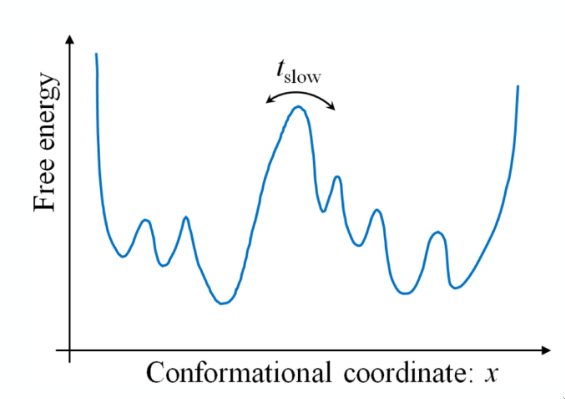
\includegraphics[width = \textwidth]{time-scales}
		\caption{Time scales}
		\label{fig:time-scales}
	\end{figure}

	Figure \ref{fig:time-scales} depicts a free energy profile.
	Usually when starting a simulation the starting point is a minimum.
	Sampling the simulation for a long time a transition to other minima could be observed, but these processes that happen to processes that happen on a faster time-scale with respect to processes that need to surpass a higher energy barrier.
	The time-scale of the transition depends exponentially on the height of the transition, so the higher the barrier the longer the time to observe the transition.
	Whenever a simulation is started an estimate of the slowest time scale involved in the process need to be understood.



\section{Equilibration}
When performing a simulation it is fundamental to consider if the simulation is equilibrated enough, so if the system has equilibrated after the simulation.
This is very difficult to understand, but it is easy to tell if a system is non-equilibrated.
Some of the variables that can be checked to see for non-equilibration are scalar values:

\begin{multicols}{2}
	\begin{itemize}
		\item System size which depends on the ensemble: in the case of NPT it is important.
			If it is equilibrated the volume would fluctuate around an average.
		\item Membrane area for membrane proteins: when simulating a protein at the beginning the membrane adapt to the protein and after a while equilibration is reached and area per lipid does not change and so does total membrane area.
		\item Potential energy or total energy, this is expected to fluctuate around an average value.
			At the beginning it varies due to temperature or initial configuration before reaching an average, so it as equilibrated in a local minimum of an average.
		\item Temperature in the NVE ensemble, so temperature will be constant when the system is at equilibrium.
		\item Density of simulated molecules in the NPT ensemble.
		\item Pressure, not recommended because in pressure there are huge variation because it depends on the Virial, so the average value will be $1 atm$, but the fluctuation will be huge.
		\item Radius of gyration is an overall information on the protein structure.
			There is the possibility to reach the same value in different conformation, a problem that applies to other overall distance measures.
			Even if there are conformation with the same value of gyration they could be different.
			If the radius of gyration is constantly increasing or decreasing the simulation has not equilibrated yet.
		\item Configurational distance measures like RNMS, all-to-all RMSD map.
			The discussion for radius of gyration holds for this measures.
			Considering RMSD:

			$$RMSD(\vec{r}, \vec{s}) = \sqrt{\frac{1}{N}\sum\limits_{i=1}^N|\vec{r}_i-\vec{s}_i|^2}$$

			This will reach a constant value with some fluctuation.
			The all-to-all RMSD map checks the RMSD for all the conformation present in the molecular dynamics simulation, obtaining a matrix of distances that can be plotted as in \ref{all-to-all-rmsd}.
	\end{itemize}
\end{multicols}

\begin{multicols}{2}

	\begin{figure}[H]
		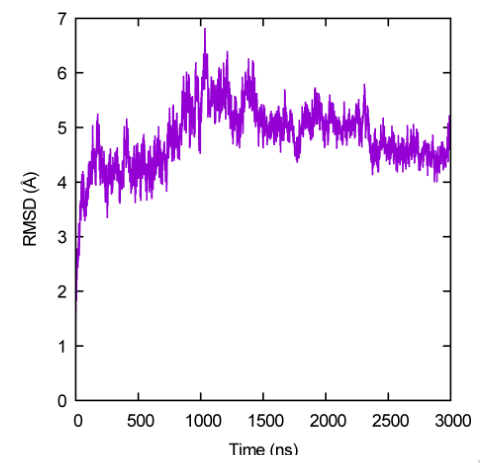
\includegraphics[width = 0.45\textwidth]{rmsd}
		\caption{RMSD}
		\label{fig:rmsd}
	\end{figure}

	\columnbreak

	\begin{figure}[H]
		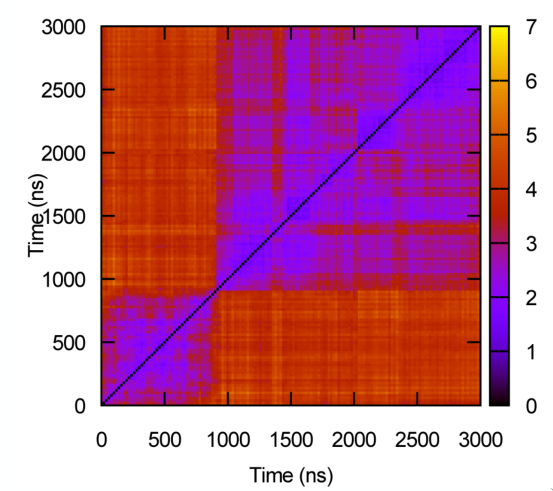
\includegraphics[width = 0.45\textwidth]{all-to-all-rmsd}
		\caption{All-to-all RMSD map, in blue low values and in red high value}
		\label{fig:all-to-all-rmsd}
	\end{figure}

\end{multicols}

It is very difficult to interpret data from \ref{fig:rmsd}, but it is easier in \ref{fig:all-to-all-rmsd}.
Looking at the latter two conformations can be seen, where there are the basins.
It can be seen how once the protein exits from the lower basin it does not come back and goes into the other.
Moreover in the bigger basis different conformation can be seen that are easily traversed.
This two basin are expected with starting with crystal's coordinate the first is the local basin corresponding to the crystal structure, which can be biased.

	\subsection{Qualitative behaviour}

	\begin{figure}[H]
		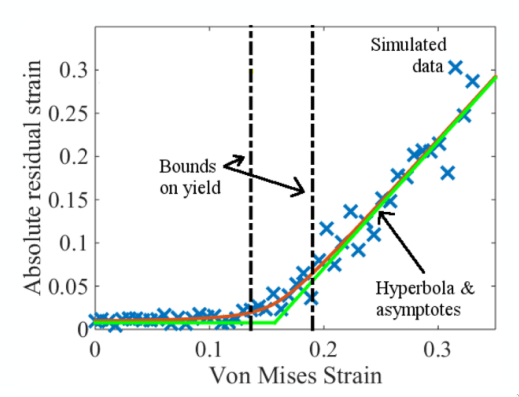
\includegraphics[width = \textwidth]{qualitative-behaviour}
		\caption{Qualitative behaviour}
		\label{fig:qualitative-behaviour}
	\end{figure}

	Knowing some qualitative features of the simulation can allow for a more constructive analysis of the data.
	Looking at \ref{fig:qualitative-behaviour} a simulation of a material is considered.
	In this case an expected behaviour is seen and then the simulated data is fitted into a known function, so in this case the expected behaviour is being reproduced, meaning that the simulation has provided good results.

	\subsection{Independent simulations}
	In principle a set of independent simulations should be run.
	Most of the time running independent simulation is not a good choice in the case of protein.
	This is because all the independent simulation are independent only in the velocities: the coordinates are the same not considering the solvent.
	This is very computational expensive, so a more efficient way would be to run long simulation starting from equilibrating structure and randomizing the velocities.

		\subsubsection{Autocorrelation analysis}
		Another method is to start from a single simulation and perform an autocorrelation analysis, to asses whether two snapshots of the simulation are independent.
		To do so the autocorrelation of two quantities like RMSD is computed:

		$$C(x_k, x_{k+j}) \equiv\frac{\bar{(x_k-\bar{x})(x_{k+j}-\bar{x})}}{s^2(x)}\Rightarrow C_j$$

		Where:

		\begin{multicols}{2}
			\begin{itemize}
				\item $x_c$ is data point at time $c$.
				\item $\bar{x}$ is the arithmetic mean.
			\end{itemize}
		\end{multicols}

		This would be done for all the $k$ values and if it does not depend by $k$ but only on $j$ the property has been equilibrated.
		If the function depends on $k$ the simulation has equilibrated.

		\subsubsection{Combined clustering}
		Combined clustering as in \ref{fig:independent_simulation}.
		In combined clustering a measure of the distance of the conformation.
		Then using one clustering algorithm the conformations will be clustered.
		There will be a number of cluster.
		Assume doing so for two independent simulations, or for two part of a long simulation, called in \ref{fig:independent_simulation} $1$ and $2$.
		Then for each of this two simulation the time the simulation spent in one cluster is computed for each cluster.
		This is plotted in the data.
		If the point are off-diagonal the trajectories are not the same so the system has not equilibrated.

		\begin{figure}[H]
			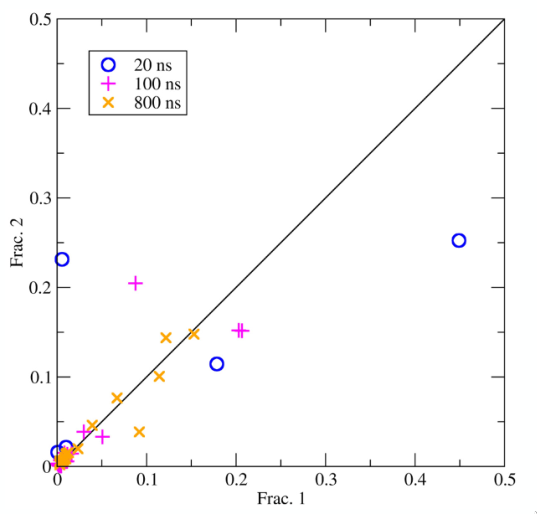
\includegraphics[width = \textwidth]{independent-simulations}
			\caption{Combined clustering}
			\label{fig:independent_simulation}
		\end{figure}

	\subsection{Equilibration and production}
	It can be seen in the case of slowly-equilibrating of figure \ref{fig:equilibration} a drift can be observed so there is no certainty of equilibration.

	\begin{figure}[H]
		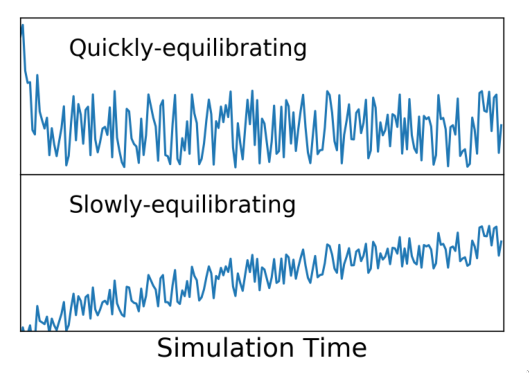
\includegraphics[width = \textwidth]{equilibration}
		\caption{Behaviour during equilibration}
		\label{fig:equilibration}
	\end{figure}

	Once we are confident that equilibration has been reached the trajectory has to be separated into the equilibration and production part.
	This can be seen in \ref{fig:equilibration-production}.
	Now equilibration is discarded and no longer considered in the analysis.
	In the analysis just the production will be considered.

	\begin{figure}[H]
		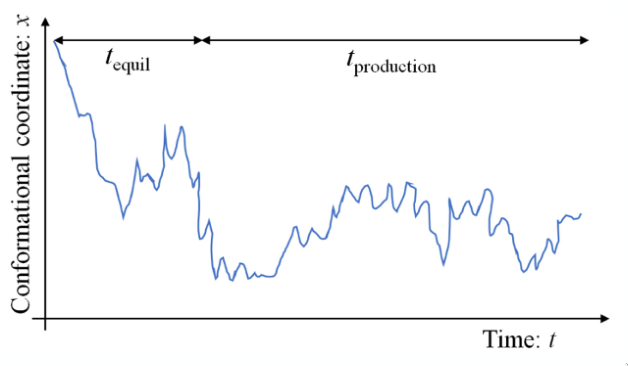
\includegraphics[width = \textwidth]{equilibration-production}
		\caption{Comparison of equilibration and production}
		\label{fig:equilibration-production}
	\end{figure}

	\subsection{Equilibration workflows}
	For the equilibration there are different type of workflow and the choice depends on the system in use.

		\subsubsection{First workflow}
		In this first workflow the simulated times are the physical time as in the NVE ensemble the Hamiltonian dynamics are considered because there is no thermostat.
		So this is a good workflow for observing dynamical properties.

		$$\overbrace{\underbrace{NVT}_{\substack{\text{short simulation to}\\\text{relax to temperature}\\\text{of interest}}}\rightarrow \underbrace{NVE}_{\text{short equilibration}}}^{\text{Suggested equilibration workflow}}\rightarrow \overbrace{NVE}^{\text{Production ensemble}}$$

		\subsubsection{Second workflow}
		In this second workflow the volume is kept fixed, the first simulation is used to adapted to the temperature and then the simulation is run.
		In this case the simulation is run at fixed density.
		This would be used for a liquid material.


		$$\overbrace{\underbrace{NVT}_{\substack{\text{short simulation to}\\\text{relax to temperature}\\\text{of interest}}}}^{\text{Suggested equilibration workflow}}\rightarrow \overbrace{\underbrace{NVT}_{\text{at known, fixed density}}}^{\text{Production ensemble}}$$


		\subsubsection{Third workflow}
		This third workflow is typical for proteins.
		So a combination of NPT and NVT to converge the volume and then the system is simulated without a barostat.

		$$\overbrace{\underbrace{NVT}_{\substack{\text{short simulation to}\\\text{relax to temperature}\\\text{of interest}}}\rightarrow \underbrace{NPT}_{\substack{\text{short simulation to}\\\text{relax to density of}\\\text{interest}}}\rightarrow\underbrace{NPT}_{\substack{\text{to compute average}\\\text{box size}}}\rightarrow \underbrace{NVT}_{\text{short equilibration}}}^{\text{Suggested equilibration workflow}}\rightarrow\overbrace{\underbrace{NVT}_{\substack{\text{for density defined by}\\\text{ pressure or unknown system}\\\text{density distribution,}\\\text{like a homogeneous system}}}}^{\text{Production ensemble}}$$

		\subsubsection{Forth workflow}
		This is a typical simulation for a membrane protein.

		$$\overbrace{\underbrace{NVT}_{\substack{\text{short simulation to}\\\text{relax to temperature}\\\text{of interest}}}\rightarrow \underbrace{NPT}_{\substack{\text{short simulation to}\\\text{relax to density of}\\\text{interest}}}}^{\text{Suggested equilibration workflow}}\rightarrow	\overbrace{NPT}^{\text{Production ensemble}}$$

\section{Autocorrelation}

	\subsection{Autocorrelation function}
	The autocorrelation function is useful to understand whether a system is equilibrated enough and how many independent conformations there are in the analysis.
	This is possible only when the correlation time is computed for an observable.
	So there is an autocorrelation function and time for each observable.
	Let $f(x)$ an observable, a function of the coordinates or the momenta.
	Then the autocorrelation function:

	$$C_f(t') = \frac{\bigl\langle(f(x)-\langle f\rangle)(f(t+t') - \langle f\rangle)\bigr\rangle}{\sigma^2_f}$$

	When $t'=0$ $C_f(t') = 1$.
	This function will decrease with $t'$.
	Using both the equilibration and production part of the simulation $C_f(t')$ will also depend on time time $t$.
	Using only the production run the dependence of $t$ is lost and the autocorrelation function can be computed.
	The function will go to $0$ with an exponential behaviour and fluctuate around that value.
	Performing this on a discretized time and the time ordered sequence of values $f_j = f(t=j\Delta t)$:

	$$C_f(t') = \frac{1}{\sigma^2_f}\frac{1}{N}\sum\limits_{j=1}^{N-\frac{t'}{\Delta t}}(f(j\Delta t)-\langle f\rangle)(f(j\Delta t + t')-\langle f\rangle)$$

	Computing the autocorrelation function starting after an increasing time if the system has equilibrated within the first time chosen the curves superimpose in the first part.

	\subsection{Autocorrelation time}
	The autocorrelation time is defined as:

	$$\tau_f = \int_0^{+\infty} dt' C_f(t')$$

	If the autocorrelation function is an exponential this is a good way to estimate the autocorrelation time.
	Looking at figure \ref{fig:autocorrelation-time}, although it seems that after $200ps$ the autocorrelation time is reached in this way the number of independent conformation is obtained.
	It could be that this number is not sufficient to sample the system properly.
	In that case the system is spending too much time in one conformation and not according to the Boltzmann distribution.
	The autocorrelation time will provide an idea on how many independent conformation there are in the syste,

	\begin{figure}[H]
		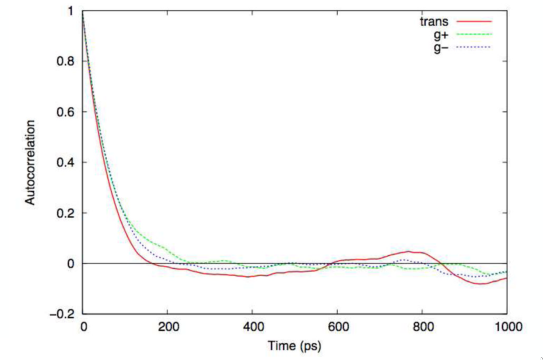
\includegraphics[width = \textwidth]{autocorrelation-time}
		\caption{Autocorrelation time}
		\label{fig:autocorrelation-time}
	\end{figure}

	The autocorrelation time $\tau_f$ is specific for each observable $f$ and allows to obtain the number of independent values of $f$ in the simulation:

	$$N_f^{ind}\simeq\frac{t_{sim}}{\tau_f}$$

	Where $t_{sim}$ is the total simulation time.
	Once the number of independent value is estimated the standard deviation of the mean can be computed using this number:

	$$SE(f) = \frac{\sigma_f}{\sqrt{N_f^{ind}}}\sim\sigma_f\sqrt{\frac{\tau_f}{t_{sim}}}$$

	A confidence interval at $95\%$ implies: $\pm 2 SE(f)$.

\section{Block averaging analysis}
The block averaging analysis is another way to compute the autocorrelation time.
In this method a trajectory with $N = M\cdot n$ snapshots is divided into $M$ segments of length $n$ with $n =1, 2, \dots$.
Compute $M$ averages, one in each block:

$$\langle f\rangle_i, \qquad i = =1, \dots, M$$

Compute the standard deviation $\sigma_n$ for each value of $n$.
Running estimate of the overall standard error:

$$BSE(f, n) = \frac{\sigma_n}{\sqrt{M}}$$

For small values of $n$ and high values of $M$, the $BSE$ under-estimates the statistical error.
The $BSE$ is constant once the blocks are essentially independent of one another, or when the block length is substantially greater than the correlation time.


\begin{multicols}{2}

	\begin{figure}[H]
		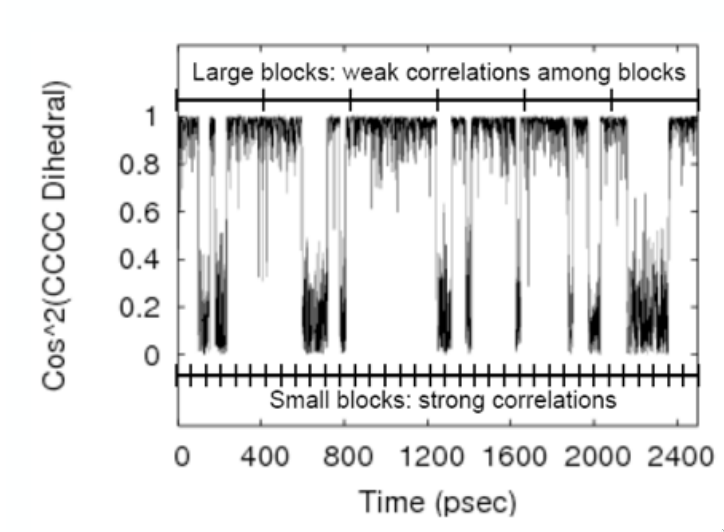
\includegraphics[width = 0.45\textwidth]{block-length}
		\caption{Varying block length}
		\label{fig:block-length}
	\end{figure}

	\columnbreak

	\begin{figure}[H]
		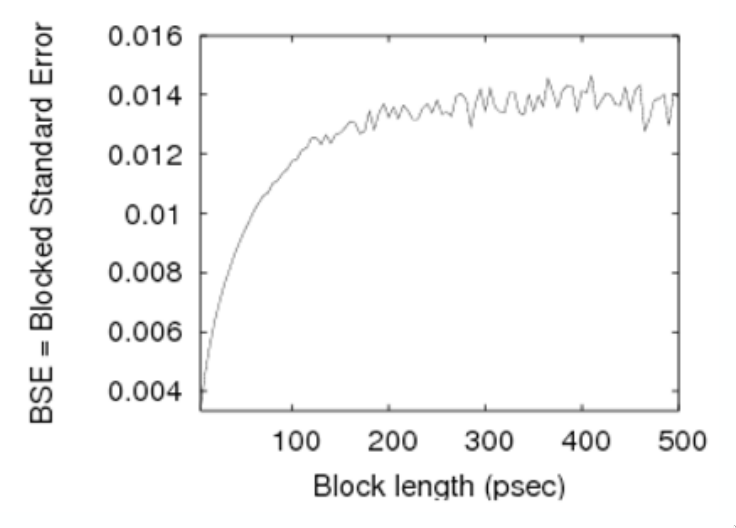
\includegraphics[width = 0.45\textwidth]{bse}
		\caption{BSE at varying block length}
		\label{fig:bse}
	\end{figure}

\end{multicols}

  \graphicspath{{chapters/15/images}}
\chapter{Protein motions}

\section{Elastic network models}

\begin{figure}[H]
	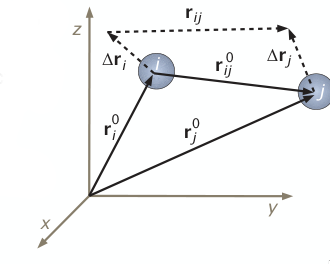
\includegraphics[width=\textwidth]{enm-theory}
	\caption{Elastic network models}
	\label{fig:kirchhoff-adjacency}
\end{figure}

Configuration vector of the protein: $\vec{r} = [\vec{r}_1, \vec{r}_2, \dots, \vec{r}_N]$.
Deviation from the equilibrium position (PDB structure):

$$\Delta\vec{r}_i = \vec{r}_i-\vec{r}_i^0$$

Instantaneous changes in the positions of all residues:

$$\Delta\vec{r} = [\Delta\vec{r}_1, \Delta\vec{r}_2, \dots, \Delta\vec{r}_N]$$


Equilibrium separation between two beads $i$ and $j$: $\vec{r}_{ij}^0 = \vec{r}_j^0-\vec{r}_i^0$.
Instantaneous separation between two beads $i$ and $j$: $\vec{r}_{ij} = \vec{r}_{ij}^0+\Delta\vec{r}_{ij}$, $\Delta\vec{r}_{ij} = \Delta\vec{r}_i-\Delta\vec{r}_i$.

\section{Gaussian network model}
Potential energy for each couple:

$$U_{ij} = \gamma_{ij}(\Delta\vec{r}_j-\Delta\vec{r}_i)\cdot(\Delta\vec{r}_j-\Delta\vec{r}_i) = \gamma_{ij}\Delta\vec{r}_{ij}^2$$

Total elastic energy:

$$U_{GNM} = \frac{1}{2}\sum\limits_i\sum\limits_j\gamma_{ij}\Delta\vec{r}^2_{ij} = \frac{\gamma}{2}\sum\limits_i\sum\limits_j\Delta\vec{r}_{ij}^2$$

Cutoff radius: $r_c = \si{\angstrom}$.

So the total potential energy:

$$U_{GNM} = \frac{\gamma}{2}\Delta\vec{r}(t)^T\Gamma\Delta\vec{r}(t)$$

Where $\Gamma$ is the Kirchoff adjacency matrix.

\begin{figure}[H]
	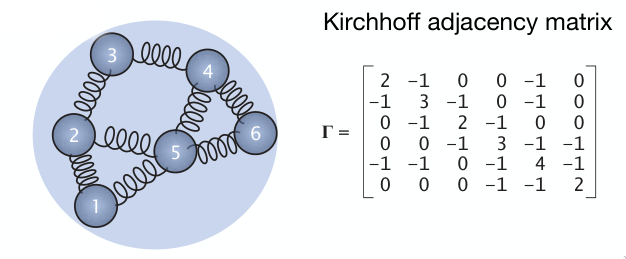
\includegraphics[width=\textwidth]{kirchoff-adjacency-matrix}
	\caption{Kirchhoff adjacency matrix}
	\label{fig:kirchhoff-adjacency}
\end{figure}

	\subsection{Correlated motions}

	$$\langle\Delta\vec{r}_i\cdot\Delta\vec{r}_j\rangle = \frac{1}{Q}\int\Delta\vec{r}_i\cdot\Delta\vec{r}_je^{-\frac{U}{kT}}d^N\Delta\vec{r}$$

	Generalized Gaussian integral:

	$$\langle\Delta\vec{r}_i\cdot\Delta\vec{r}_j\rangle = \frac{3kT}{\gamma}[\Gamma^{-1}]_{ij}$$

	Where $\Gamma^{-1}$ is a pseudoinverse matrix as the Kirchhoff matrix has zero determinant and cannot be inverted.
	Considering the eigenvalue decomposition: $\Gamma = U\Lambda U^T$:

	$$U = [\vec{u}_1, \dots, \vec{u}_{N_1}] = \begin{bmatrix} u_{1,1} & \cdots & u_{N-1,1}\\\vdots & \cdots & \vdots\\ u_{1, N} & \cdots & u_{N-1, N}\end{bmatrix}\qquad\Lambda = \begin{bmatrix} \lambda_1 & 0 & 0 & \cdots & 0\\ 0 & \lambda_2 & 0 &\cdots & 0\\0 & 0& \lambda_3 & \cdots & 0\\\vdots & \vdots & \vdots & \vdots &\vdots\\ 0 & 0 & 0 & \cdots & \lambda_{N-1}\end{bmatrix}$$

	\subsection{Gaussian network model and B-factors}

	$$\langle\Delta\vec{r}_i\cdot\Delta\vec{r}_i\rangle = \frac{3kT}{\gamma}[U\Lambda^{-1}U^{T}]_{ii} = \frac{3kT}{\gamma}\sum\limits_{k}[\lambda_k^{-1}\vec{u}_k\vec{u}_k^T]_{ii} = \sum\limits_{k}[\Delta r_i^2]_k$$

	Debye-Waller factors:

	$$B_i = \frac{8\pi^2}{3}\langle\Delta r_i^2\rangle$$

	\begin{figure}[H]
		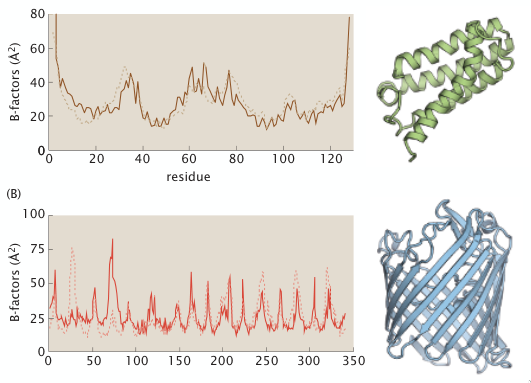
\includegraphics[width=\textwidth]{gnm-b-factors}
		\caption{GNM and B-factors}
		\label{fig:gnn-b-factors}
	\end{figure}

	\subsection{Biological relevance}

	\begin{figure}[H]
		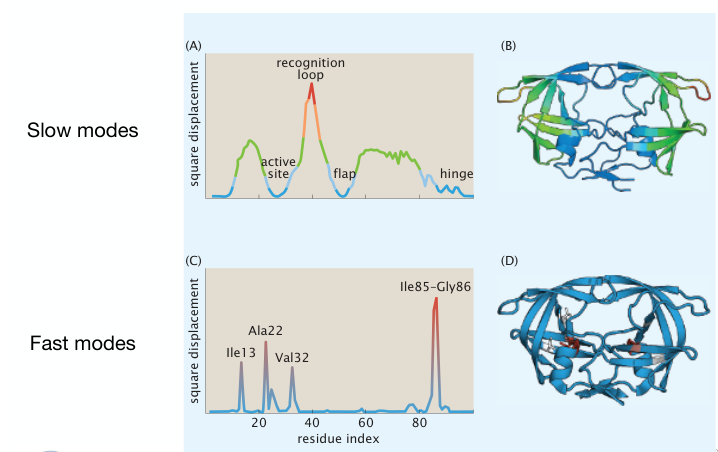
\includegraphics[width=\textwidth]{biological-relevance}
		\caption{Biological relevance}
		\label{fig:biological-relevance}
	\end{figure}

	\subsection{Normal mode analysis}

	$$U = U_0 + \sum\limits_i\frac{\partial U}{\partial q_i}|_{q^0}(q_i-q_i^0) + \frac{1}{2}\sum\limits_i\sum\limits_j\frac{\partial^2 U}{\partial q_i\partial q_j}|_{q^0}(q_i-q_i^0)(q_j-q_j^0) + \cdots$$

	At equilibrium:

	$$U = \frac{1}{2}\Delta\vec{q}^TH\Delta\vec{q} = \frac{1}{2}\sum\limits_i\sum\limits_j H_{ij}(q_i-q_i^0)(q_j-q_j^0)$$

	Hessian matrix:

	$$H_{ij} = \frac{\partial^2 U}{\partial q_i\partial q_j}|_{q^0}$$

	Covariance matrix:

	$$C = \langle\Delta\vec{q}\Delta\vec{q}^T\rangle = \frac{1}{Q}\int\Delta\vec{q}\Delta\vec{q}^Te^{-\frac{\Delta\vec{q}^TH\Delta\vec{q}}{2kT}}d^N\Delta\vec{q} = kTH^{-1}$$

  \graphicspath{{chapters/16/images/}}
\chapter{Clustering and protein structure networks}

\section{Clustering}
The aim of clustering is to find a way to group a set of data into clusters of similar properties.
This is done because:

\begin{multicols}{2}
	\begin{itemize}
		\item Labelling is expensive.
		\item To gain insight into the structure of data.
		\item Find prototypes in the data.
	\end{itemize}
\end{multicols}

In molecular simulations data usually refers to protein, DNA or RNA conformations.
So, given a set of data points, each described by a set of attributes, the clusters have to be found such that:

\begin{multicols}{2}
	\begin{itemize}
		\item Intra-cluster similarity is maximized.
		\item Inter-cluster similarity is minimized.
	\end{itemize}
\end{multicols}

	\subsection{Distance measures}
	To define similarity let $O_1$ and $O_2$ be two objects from the universe of possible objects.
	The distance or dissimilarly between $O_1$ and $O_2$ is a real number $D(O_1, O_2)$.
	A distance measure should have the following properties:

	\begin{itemize}
		\item Symmetry: $D(A,B) = D(B, A)$.
		\item Constancy of self-similarity: $D(A, A) = 0$.
		\item Positivity (separation): $(A, B) = 0\Leftrightarrow A=B$.
		\item Triangular inequality: $D(A, B) \le D(A, C) + D(B, C)$.
	\end{itemize}

	\subsection{Types of clustering}

	\begin{itemize}
		\item Hierarchical algorithms: create a hierarchical decomposition of the set of objects using some criterion.
		\item Partitional algorithms: construct various partitions and then evaluate them by some criterion,
	\end{itemize}

	\subsection{Dendrograms}
	In a dendrogram (\ref{fig:dendrogram}) the similarity between two objects is represented as the height of the lowest internal node they share.

	\begin{figure}[H]
		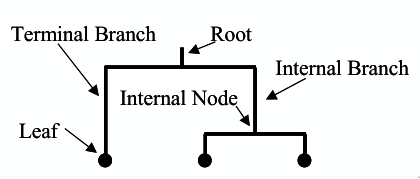
\includegraphics[width=\textwidth]{dendrogram}
		\caption{Dendrogram structure}
		\label{fig:dendrogram}
	\end{figure}

		\subsection{Interpretation}
		Hierarchical clustering sometimes show pattern that are meaningless or spurious.

\section{Correct number of clusters}

	\begin{figure}[H]
		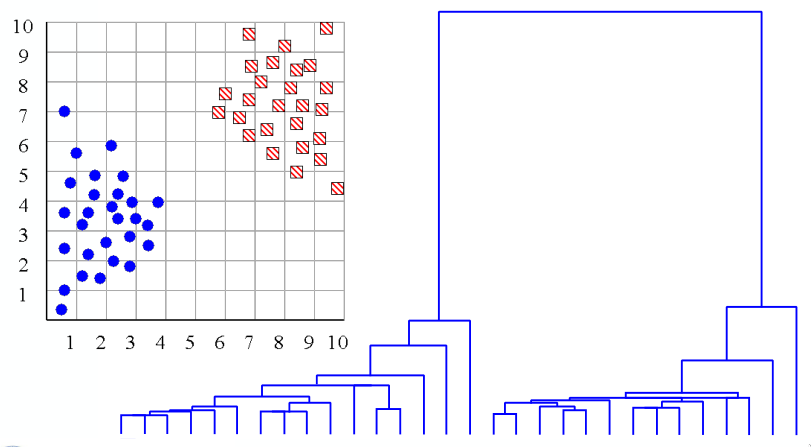
\includegraphics[width=\textwidth]{correct-number}
		\caption{Correct number of clusters}
		\label{fig:correct-number}
	\end{figure}

	\subsection{Outliers}

	\begin{figure}[H]
		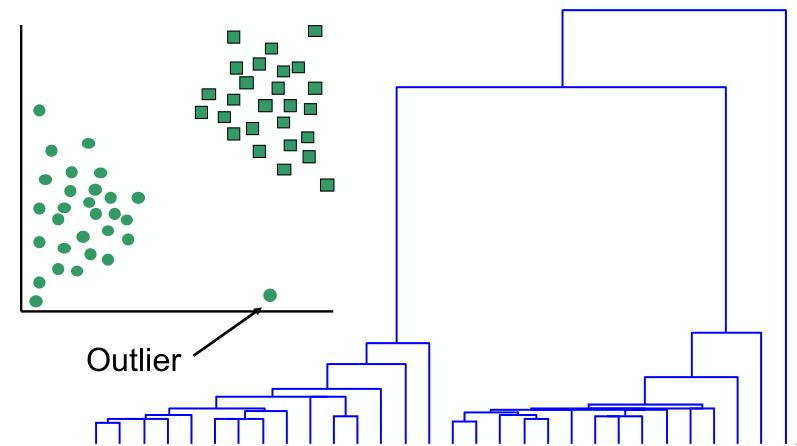
\includegraphics[width=\textwidth]{outliers}
		\caption{Outliers}
		\label{fig:dendrogram}
	\end{figure}

\section{Hierarchical clustering}
The number of dendrograms $D$ with $n$ leafs are:

$$D = \frac{2n-3)!}{2^{n-2}(n-2)!}$$

They can be built with two approaches:

\begin{itemize}
	\item Bottom-up or agglomerative approach: each item is grouped alone into its own cluster and then the best pair to merge into a new cluster is found.
		This is repeated until all clusters are fused together.
	\item Top-down or divisive approach: all the data is grouped into a single cluster, then the best division into two cluster is chosen and this is repeated recursively on both sides.
\end{itemize}

\section{Distance measures}
The distance between objects in a cluster or clusters can be computed in several ways:

\begin{itemize}
	\item Single linkage or nearest neighbour: the distance between two clusters is determined by the distance of the two closest objects (nearest neighbours) in the different clusters.
	\item Complete linkage or furthest neighbour: the distance between two clusters is the greatest distance between two objects in the different clusters.
	\item Group average linkage: the distance between two clusters is computed as the average distance between all pairs of objects in the two different clusters.
\end{itemize}

\section{Hierarchical methods}

\begin{itemize}
	\item No need to specify the number of clusters in advance.
	\item The hierarchical nature maps nicely onto human intuition for some domains.
	\item They do not scale well: $O(n^2)$.
	\item The interpretation of the results is very subjective.
\end{itemize}

\section{Partitional clustering}
In partitional clustering each item is placed in exactly one of $K$ non-overlapping clusters.
The number of cluster is provided as input.

	\subsection{K-means}

	\begin{enumerate}
		\item Choose the value $k$.
		\item Initialize the $k$ cluster centres randomly.
		\item Decide the class memberships of the $N$ objects by assigning them to the nearest cluster centre.
		\item Re-estimate the $k$-cluster centres by assuming the memberships found are correct.
		\item If non of the $N$ objects changed memberships in the last iteration exit, otherwise go back to step $3$.
	\end{enumerate}

		\subsubsection{Conclusion}

		\begin{itemize}
			\item Relatively efficient: $O(tkn)$ where $n$ is the number of objects, $k$ is the number of clusters and $t$ the number of iterations.
			\item It often terminates at a local optimum.
			\item It is applicable only when a mean can be defined.
			\item The number of cluster has to be specified in advance.
			\item It is unable to handle noisy data or outliers.
			\item It is not suitable to discover clusters with non-convex shapes.
		\end{itemize}

	\subsection{Sum of squared errors}

	$$SE_{K_i} = \sum\limits_{j=1}^m[D(C_{ij}, C_{K_i})]^2$$

	$$SE_K = \sum\limits_{i=1}^jSE_{K_i}$$

	The objective function.

	\subsection{Choosing K}
	The optimal $k$ is the one such that the $\min SE$ is found.
	It can be chosen running the algorithm with iteratively increasing value of $k$ and looking at the Knee or elbow plot of $k$ in relation with $SE$ as in \ref{fig:elbow}.

	\begin{figure}[H]
		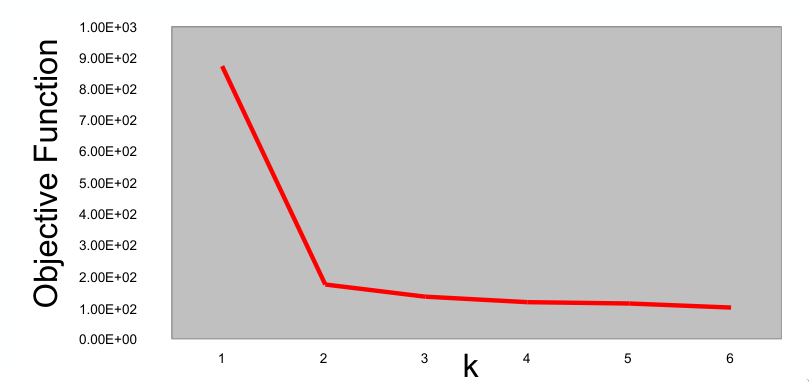
\includegraphics[width=\textwidth]{elbow}
		\caption{Knee or elbow plot}
		\label{fig:elbow}
	\end{figure}

\section{Protein structure networks}

\begin{figure}[H]
	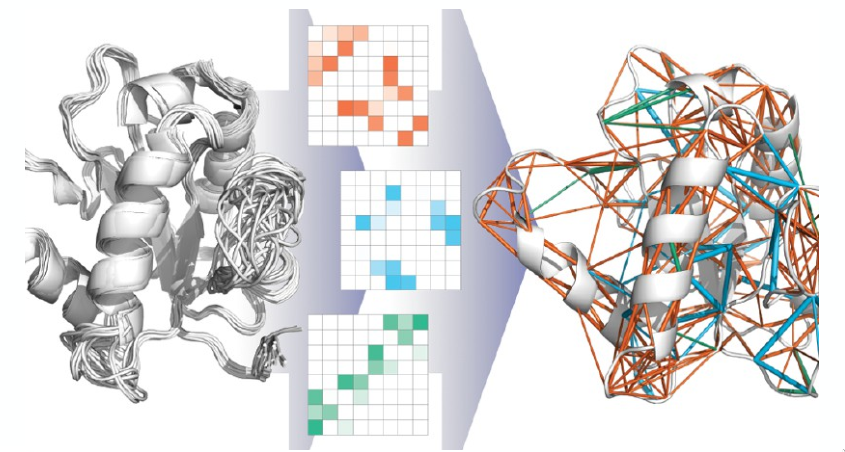
\includegraphics[width=\textwidth]{psn}
	\caption{Protein structure network}
	\label{fig:psn}
\end{figure}

	\subsection{PyInteraph}
	In PyInteraph the nodes are the side chains of protein residues.
	The edges can be defined by:

	\begin{multicols}{2}
		\begin{itemize}
			\item Distance.
			\item Atomic contacts.
			\item Van der Waals interactions.
			\item Interaction energy.
		\end{itemize}
	\end{multicols}

	Graph analysis approach to the intramolecular interaction network IIN.

	\subsection{Classes of interactions}

		\subsubsection{Hydrophobic contacts}
		In the hydrophobic contacts the centre of mass of the two side chains are distant less than $5\si{\angstrom}$.
		The centres of mass is specified by the force field for different masses.
		It has default residues:

		\begin{multicols}{4}
			\begin{itemize}
				\item Ala.
				\item Ile.
				\item Val.
				\item Phe.
				\item Met.
				\item Trp.
				\item Pro.
			\end{itemize}
		\end{multicols}

		\subsubsection{Salt bridges}
		Salt bridges are formed between atom pairs belonging to two charged groups of two different residues with distance less than $4.5\si{\angstrom}$.

		\subsubsection{Hydrogen bonds}
		Hydrogen bond happen when the distance between the acceptor and the hydrogen atom is less than $3.5\si{\angstrom}$ and the donor-hydrogen-acceptor angle is greater than $120^\circ$.

	\subsection{Persistence}
	Persitence is the fraction of the number of structures in the ensemble in which the interaction was observed.
	The Edge weight is the persistence value.
	For hydrogen-bond one or more interactions may exist between two residues.

		\subsection{Persistence threshold}
		A connected component is a subgraph in which a path exists between any two vertices, but no path exist to any other vertices of the main graph: there are no edges connecting two connected components.

	\subsection{Graph analysis}

	\begin{itemize}
		\item Highly connected residues or hubs with more than $3$ or $4$ edges allow the creation for a list of hubs and the connectivity degree for each of them.
		\item Connected components.
		\item Shortest path between two specified residues.
	\end{itemize};

	\subsection{Examples}

		\subsubsection{p53 DNA binding domain}
		Hydrophobic interactions play a crucial role in the stabilization of the protein core and in the maintenance of the 3D structure and stability.

		\begin{figure}[H]
			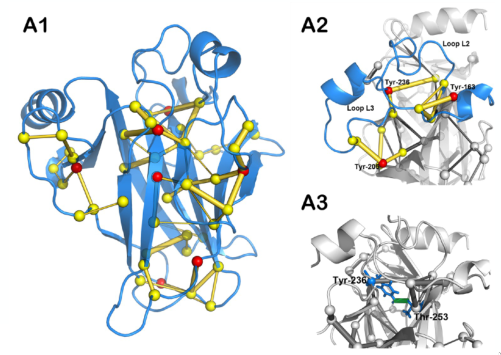
\includegraphics[width=\textwidth]{p53}
			\caption{p53}
			\label{fig:p53}
		\end{figure}

		\subsubsection{Vibrio proteinase (VAP)}
		Salt bridges or hydrogen bonds are highly flexible and cooperatively organized in networks across the protein structure for temperature adapted organisms.

		\begin{figure}[H]
			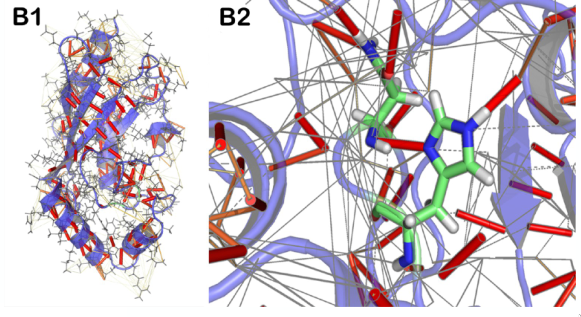
\includegraphics[width=\textwidth]{vap}
			\caption{VAP}
			\label{fig:vap}
		\end{figure}

  \graphicspath{{chapters/17/images/}}
\chapter{Monte Carlo methods}

\section{Introduction}
Monte Carlo methods are based on games of chance.
Trying to evaluate the following integral:

$$I = \int_0^1dx\int_0^{\sqrt{1-x^2}}dy = \frac{\pi}{4}$$

	\subsection{Central limit theorem}
	Let $f$ be an arbitrary function such that:

	$$f(x)\ge 0\qquad \int f(x)dx = 1$$

	And:

	$$I = \int dx\phi(x)f(x)\equiv\langle\phi\rangle_f$$

	Let $x_1, \dots, x_M$ n-dimensional vectors sampled from $f(x)$.
	Then by the central limit theorem:

	$$\tilde{I}_M = \frac{1}{M}\sum\limits_{i=1}^M\phi(x_i)\qquad \lim\limits_{M\rightarrow\infty}\tilde{I}_M = I$$

	$$\int dx\phi(x)f(x) = \frac{1}{M}\sum\limits_{i=1}^M\phi(x_i)\pm\frac{1}{\sqrt{M}}\bigl[\langle\phi^2\rangle_f-\langle\phi\rangle_f^2\bigr]^{\frac{1}{2}}$$

	\subsection{Sampling distributions}
	One dimensional distribution function:

	$$\int_a^bf(x)dx = 1\qquad f(x)\ge 0$$

	$$P(X) = \int_a^X f(x)dx\qquad X\in[a,b]$$

	$P(X)$ is the probability that any chosen $x$ from the distribution $f(x)$ lies in $[a, X]$.
	$P(X)$ is a monotonically increasing function of $X$:

	$$f(X) = Fraec{dP}{dX}$$

	Variable transformation $x\rightarrow y$ with $y = g(x)$ non decreasing function of $x$:

	$$X\ge x \Rightarrow g(X) \ge g(x)$$

	$\tilde{P}(Y=g(X))$ is the probability that $g(X)\ge g(x)$, the probability that $X\ge x$.

	$$\tilde{P}(Y) = P(X)$$

	$$w(r) = \begin{cases}1 &0\le r\le 1\\0 &otherwise\end{cases}\qquad W(\xi) = \int_0^\xi w(r)ds = \begin{cases}0 & \xi<0\\\xi & 0\le\xi\le1\\1 &otherwise\end{cases}$$

	$W(`x) = \xi$ is the probability that $r$ chosen randomly lies in $[0, \xi]$.
	$r = g(x)$ with $g(x)$ a non decreasing function: solve $P(X) = \xi$.

		\subsubsection{An example}

		$$f(x) = ce^{-cx}\qquad x\in[0, +\infty[$$

		$$P(X) = \int_0^Xce^{-cx}dx = 1- e^{-cX} = \xi\Rightarrow X = -\frac{1}{C}\ln(1-\xi)$$

		The same procedure can be generalized to more than one random variable easily when $f(x)$ is separable into a product of $n$ single-variable distributions.

	\subsection{Importance sampling}

	$$I = \int dx\phi(x)f(x) = \int dx\biggl[\frac{\phi(x)f(x)}{h(x)}\biggr]h(x) = \int dx\psi(x)h(x)$$

	$$I = \int dx\psi(x)h(x) = \frac{1}{M}\sum\limits_{i=1}^M\psi(x_i)\pm\frac{1}{\sqrt{M}}[\langle\psi^2\rangle_h-\langle\psi\rangle_h^2]^{\frac{1}{2}}$$

	This is done because $h(x)$ might be easier to sample or it might behave better than $f(x)$.
	The optimal choice for $h(x)$:

	$$\sigma^2[h] = \int dx\psi^2(x)h(x) - \biggl[\int dx\psi(x)h(x)\biggr]^2 = \int dx\frac{\phi^2(x)f^2(x)}{h(x)}-\biggl[\int dx\phi(x)f(x)\biggr]^2$$

	Minimize $\sigma^2[h]$ with the constraint $\int dx h(x) = 1$.
	Lagrange multiplier: $F[h] = \sigma^2[h]-\lambda\int dxh(x)$.
	Functional derivative: $\frac{\delta F[h]}{\delta h(x)} = 0$ with $\delta F[h] = F[h+\delta h]-F[h]$.
	Now:

	\begin{align*}
		\delta F[h] &= \int dx\biggl[\frac{\phi^2(x)f^2(x)}{h(x) + \delta h(x)} - \frac{\phi^2(x)f^2(x)}{h(x)}\biggr]-\lambda\delta h(x)=\\
								&=-\frac{\phi^2(x)f^2(x)}{h^2(x)}\delta h(x)-\lambda\delta h(x)
	\end{align*}

	$$\frac{\delta F[h]}{\delta h(x)} = 0\Rightarrow\frac{\phi^2(x)f^2(x)}{h^2(x)}+\lambda = 0\Rightarrow h(x) = \frac{1}{\sqrt{-\lambda}}\phi(x)f(x)$$

	The optimal choice: $h(x) = \frac{\phi(x)f(x)}{I}\Rightarrow \sigma^2[h] =0$.
	$I$ need to be provided.

		\subsubsection{An example}

		$$\int_0^1 dxe^{-x}$$

		\begin{figure}[h]
			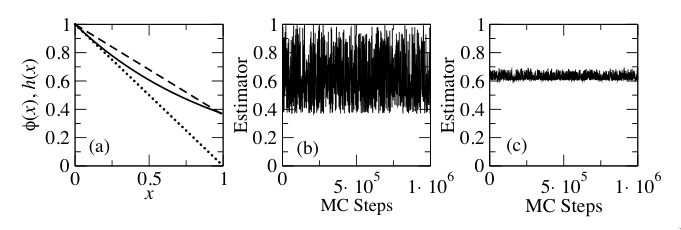
\includegraphics[width=\textwidth]{importance-sampling}
			\caption{The integrand and two possible importance functions}
			\label{fig:importance-sampling-example}
		\end{figure}

\section{Markov chains}

$$\tilde{I}_M = \frac{1}{M}\sum\limits_{i=1}^M\phi(x_i)$$

The vectors $x_1, x_2, \dots, x_M$ can be generated sequentially in a Markov chain: a rule to generate $x_{i+1}$ given $x_i$ is given.
$R(x|y)$ is the probability to obtain $x$ given $y$.
If there are two micro states it is the probability to move to a microstate $x$ from a microstate $y$.
Detailed balance condition:

$$R(x|y)f(y) = R(y|x)f(x)$$

\begin{itemize}
	\item Microscopic reversibility.
	\item Unbiased sampling of phase space.
	\item Sufficient but not strictly necessary condition to ensure proper sampling of phase space.
\end{itemize}

	\subsection{Rejection methods}
	$T(x|y)$ is a rule to generate a trial move or proposed move from $y$ to $x$.
	Normalization:

	$$\int dxT(x|y) = 1$$

	$A(x|y)$ is the probability to accept the move from $y$ to $x$:

	$$R(x|y) = A(x|y)T(x|y)$$

	By applying the detailed balance condition:

	$$A(x|y)T(x|y)f(y) = A(y|x)T(y|x)f(x)$$

	The acceptance probabilities are related.

	$$A(x|y) = \frac{T(y|x)f(x)}{T(x|y)f(y)}A(y|x) = r(x|y)A(y|x)$$

	If $A(x|y) = 1$ the move $y\rightarrow x$ is favoured $\Rightarrow A(y|x)< 1 \Rightarrow r(x|y)>1$.
	If $A(x|y) < 1$, $y\rightarrow x$ is not entirely favoured $\Rightarrow A(y|x) = 1\Rightarrow r(x|y) < 1$.

	$$A(x|y) = \min[1, r(x|y)]$$

	\subsection{Metropolis algorithm}
	The trial distribution $T(x_{k+1}|x_k)$ is used to propose a move $x_k\rightarrow x_{k+1}$:

	$$r(x_{k+1}|x_k) = \frac{T(x_k|x_{k+1})f(x_{k+1})}{T(x_{k+1}|x_k)f(x_k)}$$

	If $f(x_{k+1}|x_k)>1$ accept the move, otherwise accept the move with probability given by $r(x_{k+1}|x_k)$: extract a random number $\xi\in[0,1]$.
	If $\xi< r(x_{k+1}|x_k)$ accept the move.
	Associated probability for each point $x_1, \dots, x_n$: $\pi_1(x), \dots, \pi_n(x)$.

	$$\lim\limits_{n\rightarrow\infty}\pi_n(x) = f(x)$$

	Proof by recursive relation: $\pi_{n+1}(x)$ receives contributions from accepted moves starting at $y$ and ending in $x$ and from attempted moves to $y$ that are rejected:

	$$\pi_{n+1}(x) = \int A(x|y)T(x|y)\pi_n(y)dy + \pi_n(x)\int[1-A(y|x)]T(y|x)dy$$

	If $\pi_n(x) = f(x)$:

	$$\pi_{n+1} = \int A(x|y)T(x|y)f(y)dy + f(x)\int[1-A(y|x)]T(y|x)dy$$

	Detailed balance condition: $A(x|y)T(x|y)f(y) = A(y|x)T(y|x)f(x)$:

	$$\pi_{n+1}(x) = f(x)\int T(y|x)dy = f(x)$$

		\subsubsection{Summary}

		$$r(x|y) = \frac{T(y|x)f(x)}{T(x|y)f(y)}$$

		For a uniform choice of $T(x|y)$:

		$$r(x|y) = \frac{f(x)}{f(y)}\Rightarrow A(x|y) = \min\biggl[1, \frac{f(x)}{f(y)}\biggr]$$

	\subsection{Canonical distribution}

	$$Q(N, V, T) = \frac{1}{N!\lambda^{3N}}\int d\vec{r}_1\cdots d\vec{r}_Ne^{-\beta U(\vec{r}_1, \dots, \vec{r}_N)}$$

	$$A(r'|r) = \min\bigl[1, e^{-\beta(U(r')-U(r))}\bigr]$$

	$\Delta U < )$ accept the move.
	$\Delta U > 0$ accept the move with probability $e^{-\beta\Delta U}$.
	A Monte Carlo pass is equivalent to $N$ trial moves: particles must be chosen randomly.
	In one Monte Carlo pass each particle on average has seen one attempt.
	It is not necessary to recompute $U(r')$ in full at each move.

	$$\begin{cases}x'_i = x_i+\frac{1}{\sqrt{3}}(\xi_x-0.5)\Delta\\y'_i = y_i+\frac{1}{\sqrt{3}}(\xi_y-0.5)\Delta\\z'_i = z_i+\frac{1}{\sqrt{3}}(\xi_z-0.5)\Delta\end{cases}$$

	$\Delta$ must be chosen.

\section{Molecular dynamics and Monte Carlo methods}
In molecular dynamics:

\begin{multicols}{2}
	\begin{itemize}
		\item All particles move at once $\Delta t$.
		\item Information on dynamics.
		\item Parallel architectures.
	\end{itemize}
\end{multicols}

In Monte Carlo:

\begin{multicols}{2}
	\begin{itemize}
		\item There is no limit on the range of moves.
		\item Natural thermostats and barostats.
		\item Flexibility.
		\item Egodicity.
	\end{itemize}
\end{multicols}

	\subsection{Isothermal-isobaric ensemble}

	$$\delta(N, P, T) = \frac{1}{V_0} \int dVe^{-\beta PV}Q(N, V, T) = \frac{1}{V_0}\frac{1}{N!\lambda^{3N}}\int_0^{\infty}dVe^{-\beta PV}\int_Vd\vec{r}_1\cdots d\vec{r}_Ne^{-\beta U(\vec{r}_1, \dots, \vec{r}_N)}$$

	Previous scheme and trial moves on volume: $V' = V + (\xi_V-0.5)\delta$.
	Volume changes imply scaling of particle coordinates: $r'_i = \biggl(\frac{V'}{V}\biggr)^{\frac{1}{3}}r_i$.

	$$\Delta(N, P, T) = \frac{1}{V_0}\frac{1}{N!\lambda^{3N}}\int_0^{\infty}dVV^Ne^{-\beta PV}\int_Vd\vec{s}_1\cdots d\vec{s}_Ne^{-\beta U(V^{\frac{1}{3}}\vec{s}_1,\dots, V^{\frac{1}{3}}\vec{s}_N)}$$

	$$A(V'|V) = \min\bigl[1, e^{-\beta P(V'-V)e^{N\ln \frac{V'}{V}}e^{-\beta(U(r')-U(r))}}\bigr]$$

	$\delta$ should be small to accept the move.
	This is computational demanding, it less frequent with higher acceptance.

	\subsection{Gran canonical ensemble}

	$$\mathcal{E}(\mu, V, T) = \sum\limits_{N=0}^{\infty}e^{\beta\mu N}Q(N, V, T) = \sum\limits_{N+0}^{\infty}e^{\beta\mu N}\frac{1}{N!\lambda^{3N}}\int d\vec{r}_1\cdots d\vec{r}_Ne^{-\beta U(\vec{r}_1, \dots, \vec{r}_N)}$$

	This is the previous scheme with trial moves with particle insertion and particle deletion.
	Particle insertion:

	$$A(N+1|N) = \min\biggl[1, \frac{V}{\lambda^3(N+1)}e^{\beta\mu}e^{-\beta(U(r')-U(r))}\biggr]$$

	Particle deletion:

	$$A(N-1|N) = \min\biggl[1, \frac{\lambda^3V}{V}e^{-\beta\mu}e^{-\beta(U(r')-U(r))}\biggr]$$

	This is not so expensive: $U(r')$ requires only the change in energy due to one particle.

	\subsection{Hybrid Monte Carlo}
	Molecular dynamics is used as an engine to generate Monte Carlo moves:

	$$A(r', p' | r, p) = \min\{1, e^{-\beta[\mathcal{H}(r', p')-\mathcal{H}(r, p)]}\} = \min\bigl[1,e^{-\beta\Delta\mathcal{H}}\bigr]$$

	Symplectic time-reversible algorithm:

	$$T(r', p'|r, p) = T(r, -p|r', -p')$$

	One move is quite expensive, so it is better to have a higher acceptance rate between $40$ and $70\%$.
	In the case of a rejected move $p$ is resampled.
	If the integrator is time-reversible the detailed balance holds.

		\subsubsection{Detailed balance}
	Detailed balance condition:

		$$\int d^Npd^Np' T(r',p'|r,p)A(r',p'|r,p)f(r,p) = \int d^Npd^Np'T(r, p|r',p;)A(r,p|r',p')f(r',p')$$

		$$A(r',p'|r,p)f(r,p) = \frac{1}{Q_N(V, T)}\min\bigl[1, e^{-\beta(\mathcal{H}(r', p')-\mathcal{H}(r,p))}\bigr]e^{-\beta\mathcal{H}(r, p)}$$

		$$A(r',p'|r,p)f(r,p) = \frac{1}{Q_N(V, T)}\min\bigl[e^{-\beta\mathcal{H}(r, p)}, e^{-\beta\mathcal{H}(r', p')}\bigr]$$

		Similarly:

		$$A(r,p|r',p')f(r,'p') = \frac{1}{Q_N(V, T)}\min\bigl[e^{-\beta\mathcal{H}(r', p')}, e^{-\beta\mathcal{H}(r, p)}\bigr]$$

		Therefore: $A(r', p'|r, p)f(r, p) = A(r, p|r', p')f(r',p')$

		\subsubsection{Sympectic time-reversibility}
		Symplectic time-reversible algorithm:

		$$T(r', p'|r, p) = T(r, -p|r', -p')$$

		$$\int d^Npd^Np'T(r',p'|r, p)A(r', p'|r, p)f(r,p) = \int d^Npd^Np'T(r, -p|r', -p')A(r, p|r', p')f(r', p')$$

		Performing a change of variables: $p, p'\rightarrow -p, -p'$:

		$$\int d^Npd^Np'T(r',p'|r, p)A(r', p'|r, p)f(r,p) = \int d^Npd^Np'T(r,p|r', p')A(r, p|r', p')f(r',p')$$

  \chapter{Free energy calculations}


\end{document}
